%% 美赛模板:正文部分

\documentclass[12pt]{article}  % 官方要求字号不小于 12 号,此处选择 12 号字体

% 本模板不需要填写年份,以当前电脑时间自动生成
% 请在以下的方括号中填写队伍控制号
\usepackage[2308932]{easymcm}  % 载入 EasyMCM 模板文件.
\usepackage{listings}
\usepackage{xcolor}
\usepackage{booktabs}


% \usepackage{algorithm}
% \usepackage{algorithmicx}
% \usepackage{algpseudocode}
% \usepackage{amsmath}
% \floatname{algorithm}{Algorithm}
% \renewcommand{\algorithmicrequire}{\textbf{Input:}}
% \renewcommand{\algorithmicensure}{\textbf{Output:}}

\usepackage[linesnumbered,ruled,vlined]{algorithm2e}

\usepackage{pythonhighlight}
\usepackage{graphicx}
\usepackage{subfigure}
\usepackage{colortbl}
\usepackage{threeparttable}
\problem{A}  % 请在此处填写题号
\usepackage{mathptmx}  % 这是 Times 字体,中规中矩 
% 这是 COMAP 官方杂志采用的更好看的 Palatino 字体,可替代以上的 mathptmx 宏包
% \usepackage{mathpazo}  


\title{Raise Dragons On Earth}  % 标题

% 如需要修改题头(默认为 MCM/ICM),请使用以下命令(此处修改为 MCM)
%\renewcommand{\contest}{MCM}
\newenvironment{shrinkeq}[1]
{ \bgroup
	\addtolength\abovedisplayshortskip{#1}
	\addtolength\abovedisplayskip{#1}
	\addtolength\belowdisplayshortskip{#1}
	\addtolength\belowdisplayskip{#1}}
{\egroup\ignorespacesafterend}
% 文档开始
\begin{document}

% 此处填写摘要内容
\begin{abstract}
Dragons, the gigantic creatures form \textit{Game of Thrones}, are not found in the real world, which makes it to some extent meaningful to seriously consider what role would they play once invited into this world. By stepwise modeling, our team builds several scientific models to simulate the dragons' biological attributes, energy consumption, and their interaction with the environment.

In summary, we build three models to solve the problem. The first model estimates the energy metabolism of dragons, and in the second model, we focus our attention on the growth of the pasture, which is employed to use large-scale sheep farming to provide the necessary energy source for the dragons. The third module portrays the relationship between dragon and community. After accomplishing these, we do the implementation and explore the answers to all six tasks. Besides, we do the sensitivity analysis to check the robustness of the modules.

Firstly, we build the Metabolism of dragons. This model aims to provide an in-depth analysis of the energy needs of dragons. By considering factors such as the dragon's age, size, weight, and environment, we aim to gain a better understanding of the energy required for a dragon to grow, maintain survival, breathe fire, and fly. What's more, this model lay the foundation for our deeper analysis of how to serve the dragons better.

Secondly, we used the predator-predator model to build a sheep herding model to ensure the dragon's food source, and quantitatively evaluated the number of sheep that the pasture could support from three factors: temperature, humidity, and light conditions. We chose the actual grassland to verify the theory, and the degree of compliance was up to $95\%$. 

Nest, based on the first two established models, a community service model of the dragon is established, which takes into account the living space, food sources, and employment of the dragon, and compares the services that the dragon needs to provide in war years and normal breeding conditions. We chose three real-world grasslands in different temperature zones to fully describe the supplies dragons need in arid, temperate, and Arctic regions. 

After these efforts, we take command of the above three modules and give our answer to the six tasks of the problem. For task 1\&2, we reach our conclusion through the previous investigation of papers and the original. On the basis of our three modules, we give our answers to task 3\&4\&5. As for task 6, we compare our module results in different climates to display the importance of climate in our modules. what's more, under the guidance of this test method, we designed our sensitivity analysis, which specifically takes humidity and temperature into consideration. The result shows the robustness of our modules.

Finally, we complete the letter to be sent to George R.R. Ma, the author of \textit{ A Song of Ice and Firez}. We submit a series of suggestions in the area of how to raise the three dragons in his book in our world based on the exploration of our above models. We hope our advice can help this creative person depicts the magical world more precisely and bring better immmersiveness.

% 美赛论文中需注明关键字。若您一定要使用,
% 请将以下两行的注释号 '%' 去除,以使其生效
 \noindent\textbf{Keywords}: Dragon, Metabolism Of Dragon, Pasture Growth Model, Energy Flow, Community, Climate

\end{abstract}

\maketitle  % 生成 Summary Sheet
\tableofcontents  % 生成目录


% 正文开始
\section{Introduction}
\vspace{-0.5cm}
\subsection{Problem Background}

Dragons, legendary for their large, scaly, and winged reptiles with sharp teeth and claws, are often portrayed as having the ability to breathe burning fire or fly thousands of miles, making them the most powerful mythical creatures in the world. Typically, in George R.R. Martin’s fantasy series \textit{A Song of Ice and Fire}{\cite{11}}, the triplet dragons raised by Daeneryus Targaryen, the “Mother of Dragons.”, enjoy a great population for their strength.

Despite the fantastical elements of the story, there remains a plethora of queries regarding the practicalities of dragon husbandry that remain unaddressed. The assistance of a scientifically validated guide on the art of dragon rearing would undoubtedly augment the verisimilitude and immersiveness of this grandiose narrative, and that’s what our work aims at.



\vspace{-0.5cm}
\subsection{Restatement of Problem}
\vspace{-0.3cm}
To bring this grand creature into our world, we need to accomplish the following tasks:

$\bullet$ \textbf{Task1: }Analyzing dragons' features, behavior, habits, diet, and environmental interactions.

$\bullet$ \textbf{Task2: }Analyzing the impact and requirements dragons have on the ecosystem.

$\bullet$ \textbf{Task3: }Estimating the energy consumption and caloric intake requirements of dragons?

$\bullet$ \textbf{Task4: }Estimating the size needed to support the three dragons.

$\bullet$ \textbf{Task5: }Estimating the minimum community to sustain dragons at various levels of support.

$\bullet$ \textbf{Task6: }Evaluating the role climate conditions play in our analysis.
\subsection{Literature Review}
\vspace{-0.3cm}

In general, dragons are legendary fantasy creatures. Some scholars have analyzed a large number of historical documents{\cite{5}} and concluded that the existence of dragons is reasonable and inevitable.{\cite{1}} In addition, they even gave the corresponding laws of existence. However, there are more views that dragons are the worshipful embodiment of multi-ethnic ideology,{\cite{2}} which is also the view we hold at the time of writing this article, that is, dragons do not exist.

Armed with winged reptiles, sharp teeth, and claws, dragons are always the symbol of power, synonymous with mighty in myths. Whether it is \textit{Fafnir} in the \textit{Ring of the Nibelung}{\cite{7}} or the red dragon{\cite{6}} in the \textit{Legend Of King Arthur}{\cite{8}}, they are the top existences of the food chain in their respective legends. Most of the dragons in modern stories originated from \textit{Smaug} in the great book \textit{The Silmarillion}{\cite{9}}, and most of the dragons in later stories have the same appearance as this evil dragon. And the Targaryen family{\cite{10}} in \textit{A Song of Ice and Fire} relied on the dragon to gain the ruling power. The family motto "\textit{Fire and Blood}." may represent what dragons bring to the story: the cruelty of war and the hurt to protect peace.

The TV series Game of Thrones embodies the growth habits of dragons, which are hatched from eggs and raised by cattle and sheep. Moreover, there is no obvious difference between the three little dragons in the story except for their size. These features have similarities with lizards, birds, and ancient pterosaurs. coincides with the paper{\cite{2}}.Therefore, we believe that the feasibility of raising these three dragons in the real world exists, and the most important issue now is to collect enough food for such giant animals.

Fortunately, cattle and sheep are already in plentiful supply in this day and age, and as long as there is a suitable playground to provide adequate feed, we can feed the required amount. {\cite{12}}. But in the meantime, the balance between the environment and our feeding program must be taken seriously. Many articles focus on this{\cite{13}}{\cite{14}}{\cite{15}}, and typically, most papers concluded that low temperature, and drought is not conducive to the ecological cycle of grassland{\cite{16}}.In simpler terms, grasslands tend to flourish in regions with warm and humid climates, while cold and dry regions are not as favorable for their growth and development.

At the same time, we need to consider the purpose of the dragon when domesticating it. In the novel, the main purpose of a Lord's taming a dragon is to consolidate his power or expand his power through war. So, in our model, we divide the feeding plan of the dragon into the war phase and the breeding phase. Of course, we don't rule out the possibility of Dragons and gunships working together, even now that the weaponry is vastly improved.

Combining the pasture-sheep model of different temperature zones with different ways of using dragons, we get the final dragon serving way. And put it in the guidance letter.

\subsection{Our Work}
\vspace{-0.3cm}
To solve the above tasks, we mainly established three modules to address them. The modules include metabolism of dragon, pasture growth model and dragon's community service model. We  focus our attention on several factors, and get a series of scientific suggestions on how to raise dragons in this world.

The first model, metabolism of dragon, is designed to provide a detailed analysis of the energy metabolism of dragons, taking into account important factors such as the dragon's age, size, weight, and environmental conditions. We aim to gain a comprehensive understanding of the energy needed for the dragon to develop, maintain life, breathe fire, and fly. The model is built on scientific principles, with an emphasis on providing evidence-based, accurate assessments of a dragon's energy needs in a simple day.

The second model, pasture growth model, aims to calculate the necessary energy sources for the three dragons through raising a large number of sheep. This approach allows us to shift our focus from managing the dragons' population to maintaining ecological balance within the grazing land while satisfying their energy needs. In this model, we take into account factors such as sunlight, temperature, and humidity that affect the growth of grass. Additionally, we also consider the energy requirements of both the dragons and sheep in our calculations.

Nest, based on the above two modules, we established the dragon's community service model which takes into account the dragon's living space, food source, and their employment. By considering the difference between the services that dragons need to provide in war years and normal farming situations, we were able to optimize the dragon's role in their community. We also chose realistic pastures in three different temperature zones to comprehensively describe the supplies that dragons need in arid regions, temperate regions, and arctic regions.

\begin{figure}[htbp]
	\centering
	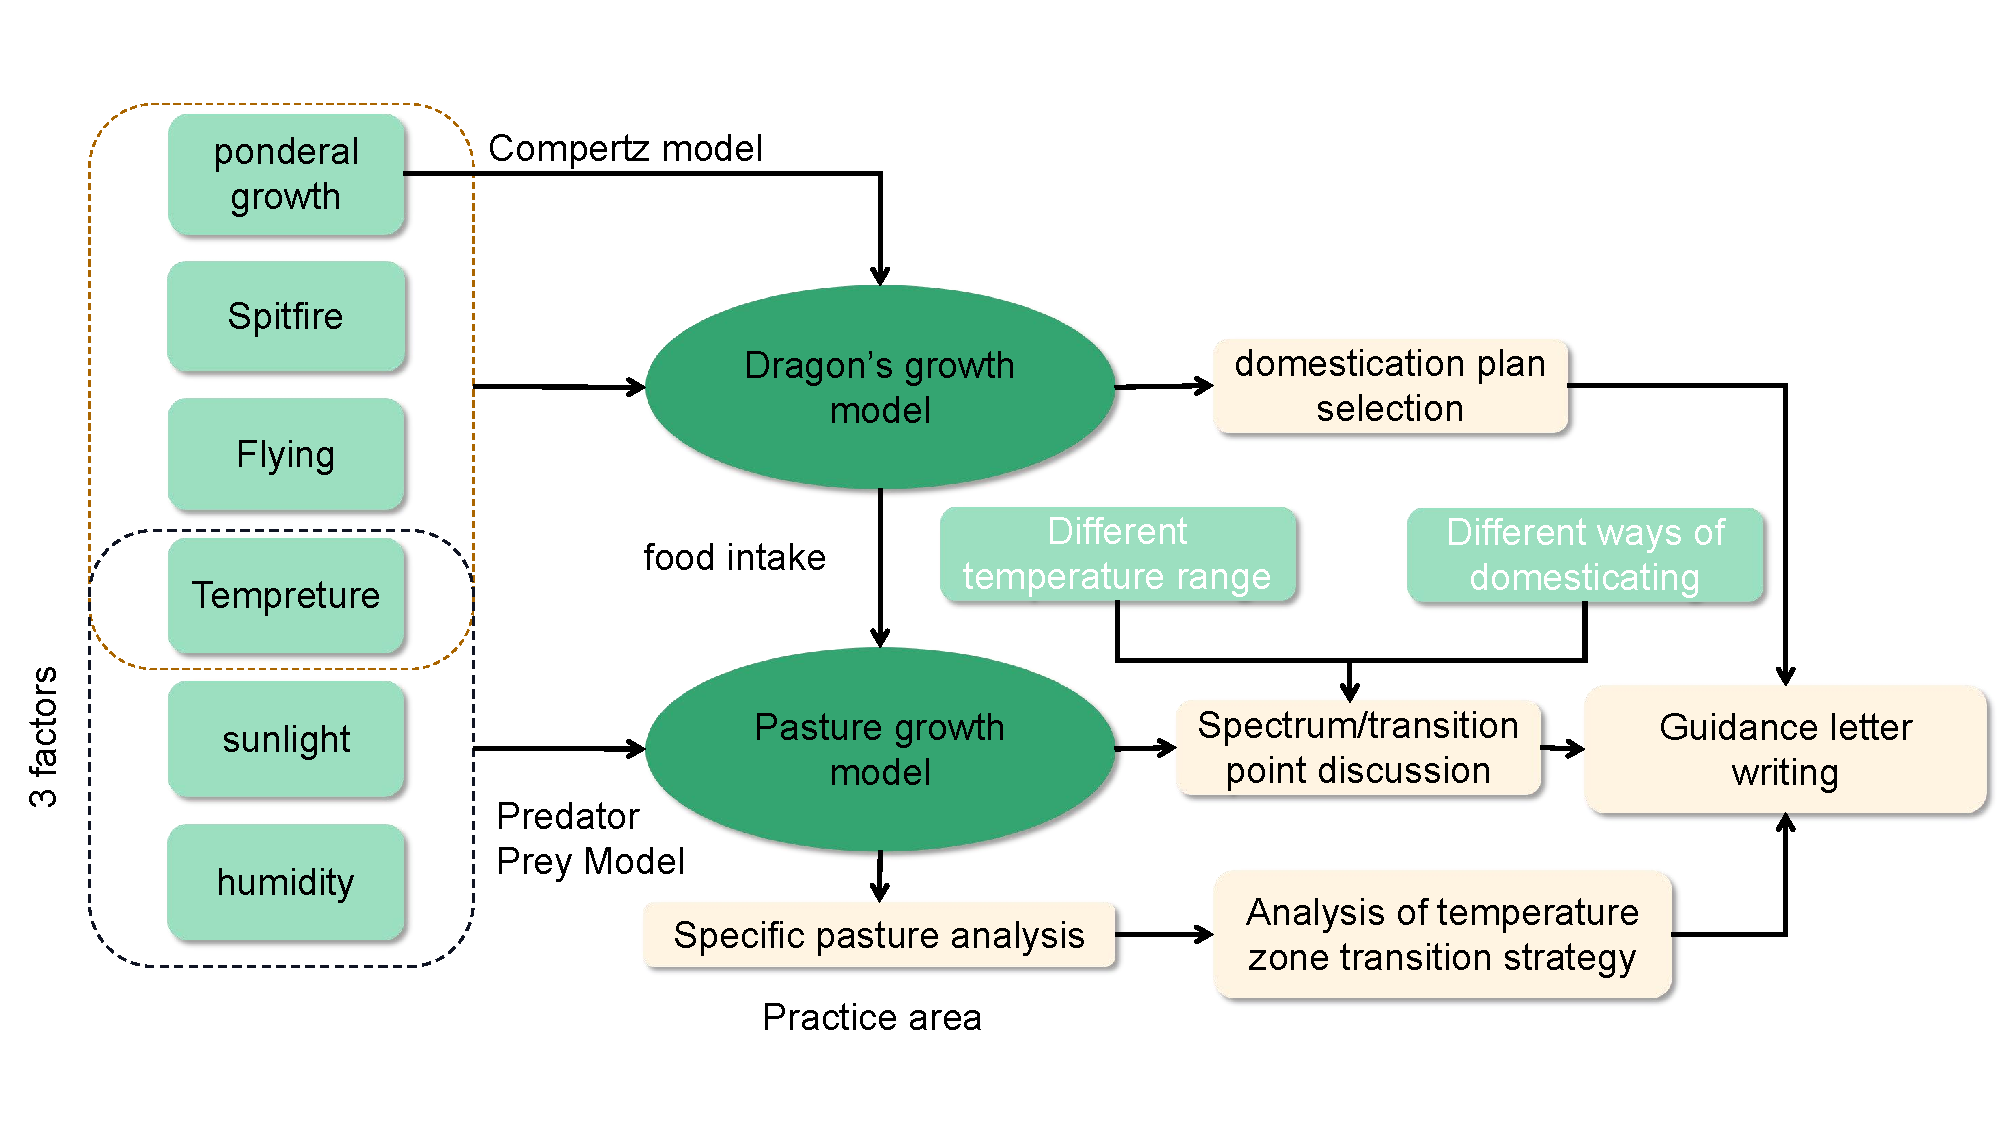
\includegraphics[width=0.85\textwidth]{frame_diagram.pdf}
	\caption{Our Work}\label{fig:pic1}
\end{figure}
\vspace{-0.3cm}

\section{Assumptions and Notations}
\vspace{-0.5cm}
\subsection{Assumptions}
\vspace{-0.3cm}

Through the full analysis of the problem, in order to simplify our model, we make the following reasonable assumptions.
\begin{itemize}
\item[$\bullet$] \textbf{Assumption1:} Dragons occupy the apex of the food chain.

\vspace{-0.2cm}
\item[$\hookrightarrow $]\textit{\textbf{Justification:}} \textit{Given the formidable offensive and defensive capabilities of dragons, we do not consider any animal to pose a significant threat to their survival.}

\item[$\bullet$] \textbf{Assumption2:} The dragon's sole purpose is twofold: to survive and participate in warfare.

\vspace{-0.2cm}
\item[$\hookrightarrow $]\textit{\textbf{Justification:}} \textit{To simplify the community model, and in reference to the role of dragons in literature, we have restricted the behavior and activities of dragons to two distinct categories: survival and warfare.}

\item[$\bullet$] \textbf{Assumption3:} In our paper, dragons are permitted to continuously grow throughout the entirety of their lives.

\vspace{-0.2cm}
\item[$\hookrightarrow $]\textit{\textbf{Justification:}} \textit{This is a hypothetical assumption derived from the premise of the question, which is corresponding to the novel.}

\item[$\bullet$] \textbf{Assumption4:} In our study, it is assumed that the three dragons possess similar attributes in terms of growth, behavior, habits, dietary needs, and other pertinent characteristics.

\vspace{-0.2cm}
\item[$\hookrightarrow $]\textit{\textbf{Justification:}} \textit{For the purpose of simplifying the model, we have only considered the possibility of three dragons having distinct growth rates, while exhibiting minimal individuality variations in other aspects.}

\item[$\bullet$] \textbf{Assumption5:} The dragons are cold-blooded oviparous creatures.

\vspace{-0.2cm}
\item[$\hookrightarrow $]\textit{\textbf{Justification:}} \textit{Drawing upon the physical characteristics of dragons as commonly depicted like komodo dragons, we have surmised that dragons are also cold-blooded, egg-laying animals.}

\item[$\bullet$] \textbf{Assumption6:} In our hypothesis, dragons are posited to utilize an internally fermented alcohol as a propellant for their fiery breath, ignited by compressing the specific gland to generate high temperatures.

\vspace{-0.2cm}
\item[$\hookrightarrow $]\textit{\textbf{Justification:}} \textit{In light of the fact that ethanol is one of the few chemical fuels that can be synthesized by enzymes within a living organism, as well as the portrayal of flames burning on water surfaces in the plot of the Battle of Blackwater, and the dragon's pre-flaming behavior of grinding its teeth, we hypothesize that dragons use ethanol, a liquid with a lower density than water, as fuel for their fire-breathing abilities, ignited through compression the specific gland.}

\item[$\bullet$] \textbf{Assumption7:} The normal lifespan of a dragon is around 200 years.

\vspace{-0.2cm}
\item[$\hookrightarrow $]\textit{\textbf{Justification:}} \textit{In the fictional world, the oldest dragon, Balerion, passed away naturally at the age of 200. Based on this, we assume that 200 years is the normal lifespan for dragons.}

\item[$\bullet$] \textbf{Assumption8:} Dragons' diet primarily consists of cattle and sheep.

\vspace{-0.2cm}
\item[$\hookrightarrow $]\textit{\textbf{Justification:}} \textit{Considering that the main food of the dragon is meat and they eat a huge amount, while beef and mutton are relatively abundant meat resources in our world, so we use beef and mutton as raw materials for raising dragons.}

\end{itemize}


\subsection{Notations}
\vspace{-0.3cm}
The primary notations used in this paper are listed in Table \eqref{tab:table_one}.
\vspace{-0.4cm}
\begin{table}[!htbp]
	\caption{Parameter Settings}
    \label{tab:table_one}
    \centering
	\begin{tabular}{ccc}
		\toprule[1.5pt]
		\makebox[0.15\textwidth][c]{\textbf{\textit{Symbols}}}	&  \makebox[0.5\textwidth][c]{\textbf{\textit{Description}}}&
        \makebox[0.15\textwidth][c]{\textbf{\textit{Unit}}}	\\
		\toprule[0.75pt]
  	$x$ & dynamic Grass production & $t$\\
    	$y$ & The number of sheep & $k$\\
        $t$ & The age of dragon & $year$\\
        $W$ & The weight of dragon & $kg$\\
        $W'$ & The weight growth per year of dragon & $kg/y$\\
        $V_a$ & Energy consumption for resting metabolism per day & $kJ$\\
        $P$ & Energy consumption for flight per day & $kJ$\\
        $V$ & Relative speed of dragon and air flow & $m/s^2$\\
        $W_{daily}$ & Energy consumption of dragon per day & $kJ$\\
		\bottomrule[1.5pt]
	\end{tabular}
\end{table}
\vspace{-0.6cm}
% \newpage

\section{Model \uppercase\expandafter{\romannumeral1} : Metabolism of dragon}
\vspace{-0.3cm}
\subsection{Model overview}
This model is geared towards providing a comprehensive evaluation of the energy metabolism of dragons. By taking into account key factors such as the dragon's age, volume, weight, and temperature conditions, we aim to gain a deeper understanding of the energy requirements for a dragon to grow, survive, breathe fire, and fly. We place a strong emphasis on scientific rigor in our modeling process, striving to make accurate, evidence-based assessments of the energy needs of dragons in the real world on a daily basis.
\subsection{Dragon growth model}
For the growth of dragons, we use the Gompertz model that best fits the growth curve of birds.

\begin{shrinkeq}{-1ex}
	\begin{equation}
    \label{eq:eq1}
	   W(t) = W_{\infty}exp[ln(\frac{W_0}{W_{\infty}}exp(-kt))]
	\end{equation}
\end{shrinkeq}

\begin{itemize}
\vspace{-0.2cm}
\item[$\bullet$] \textbf{$W$ }stands for the body weight of the animal at age $t$. 
\vspace{-0.2cm}
\item[$\bullet$] \textbf{$W_{\infty}$ }represents the mature weight (asymptote).
\vspace{-0.2cm}
\item[$\bullet$] \textbf{$W_{0}$ }is the birth weight.
\vspace{-0.2cm}
\item[$\bullet$] \textbf{$k$ }is a constant that is directly related to the postnatal rate of maturing and can be interpreted as a maturing index, establishing the rate at which $W$ approaches $W_{\infty}$.
\end{itemize}
\vspace{-0.3cm}
In this model, the birth weight of a dragon is $10kg$, and the mature weight is $75t$. Under the circumstances where $t = 1 year$, $W = 35kg$, $k =0.15 year^{-1}$.The growth curve of the model is shown below.
\begin{figure}[h]
	\centering
	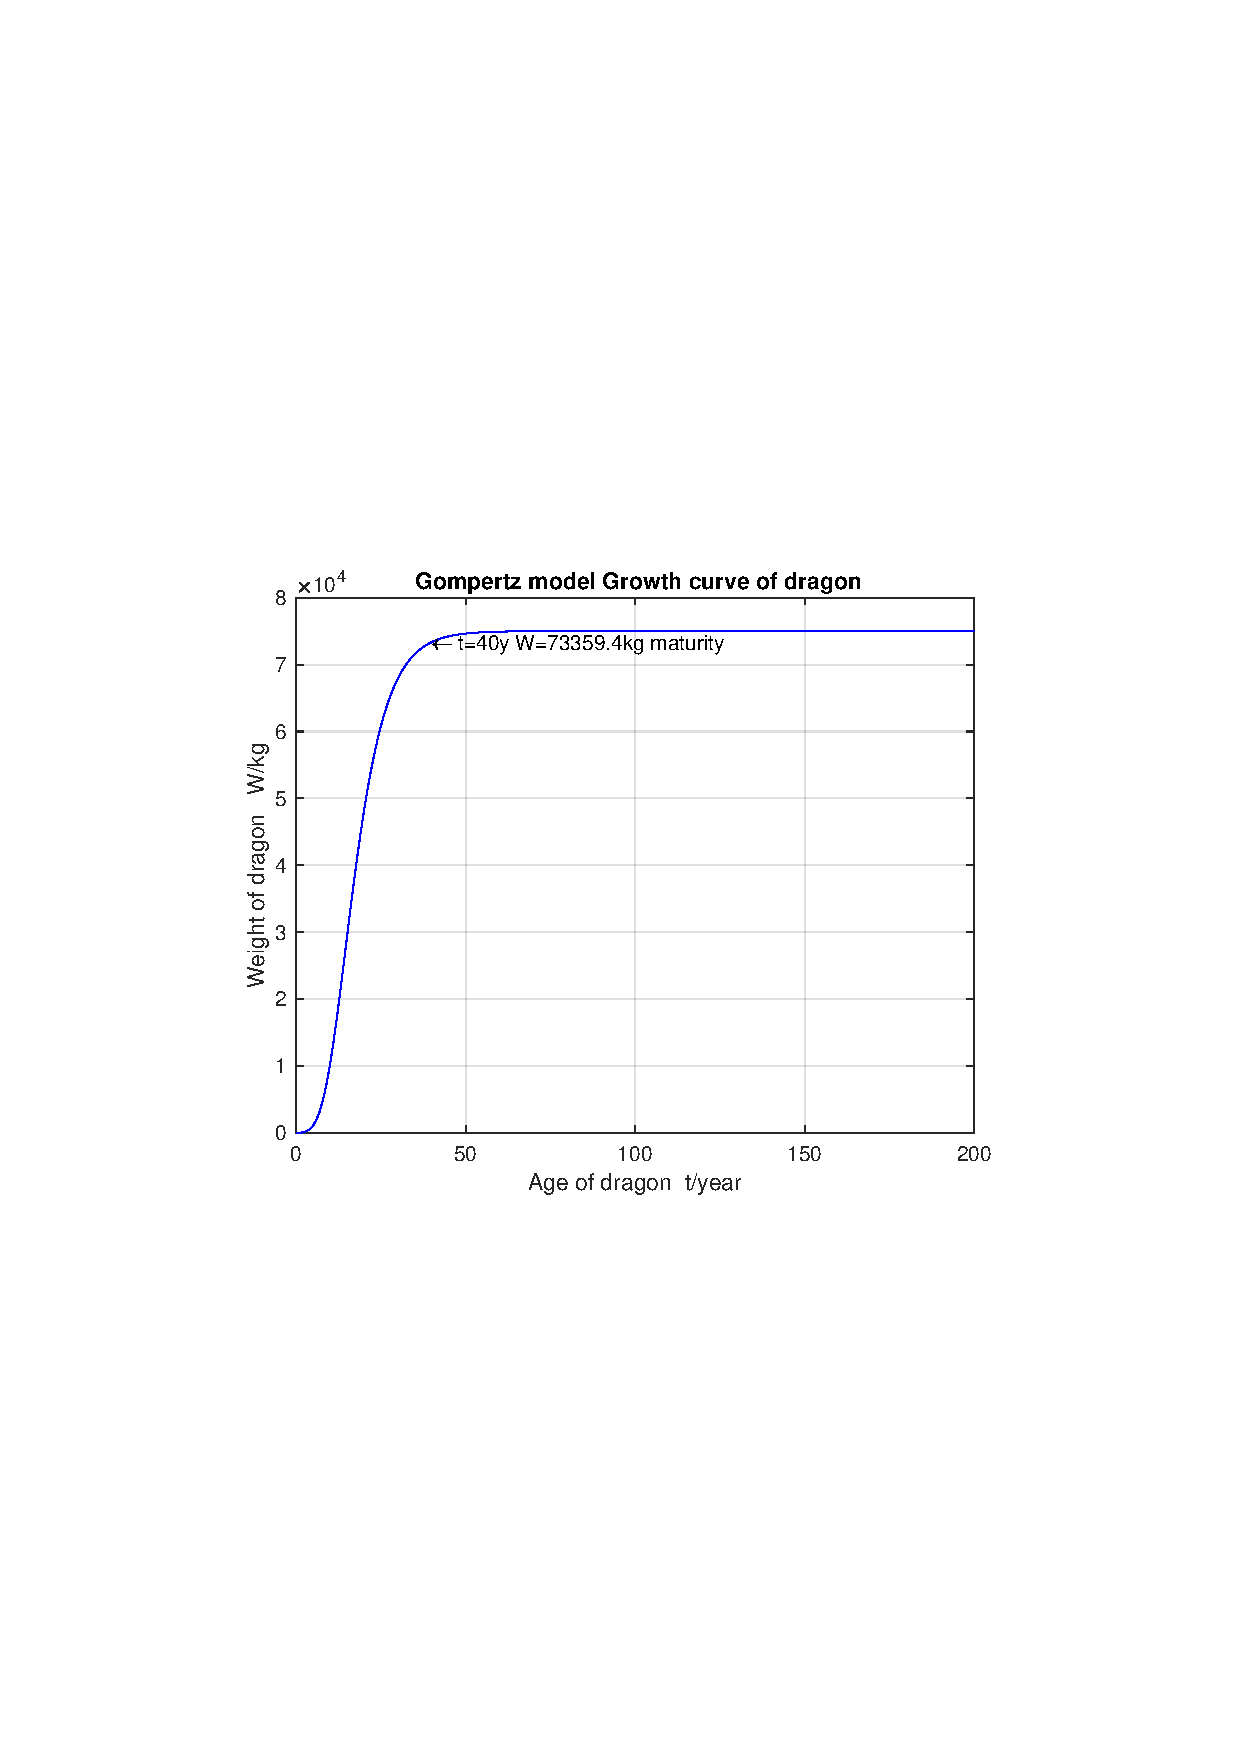
\includegraphics[width=0.5\textwidth]{easymcm/img/Gompertz model Growth curve of dragon.pdf}
	\caption{Growth curve of dragon}
\end{figure}
	
	


From this graph,We found that before the age of 40, the dragon is in a rapid growth period. At the age of about 40, the growth rate slow down and enter the mature period. The age of 40 is the point of maturity
.What's more, we are able to observe that, the weight growth per year of one dragon is  
\begin{shrinkeq}{-1ex}
	\begin{equation}
    \label{eq:eq2}
	   W' = kln(\frac{W_\infty}{W_0})Wexp(-kt)
	\end{equation}
\end{shrinkeq}

Here, We use the symbol $G$ to represent the energy required to gain $1kg$. In the meantime, we set $G = 29301 kl/kg$.

\newpage
\subsection{Fire breathing model}
We assume that the dragon has two storage pockets in its mouth, which can store the ethanol produced when fermentation occurs in the dragon's stomach. The chemical equation for the production of ethanol in the dragon's stomach is shown by the formula \eqref{eq:eq3}.


\begin{shrinkeq}{-1ex}
	\begin{equation}
    \label{eq:eq3}
	   C_6H_{12}O_6 == 2C_2H_5OH + 2CO_2 + Energy
	\end{equation}
\end{shrinkeq}

The storage bag can freely contract. When breathing fire, the storage bag rapidly contracts, due to the short compression time, this process is an adiabatic process, ethanol in the storage bag is compressed to the ignition point in a small range, then it is sprayed out through two small holes on the edge of the mouth, and burns at atmospheric pressure outside the body, which is shown in the below picture.

\begin{figure}[h]
	\centering
	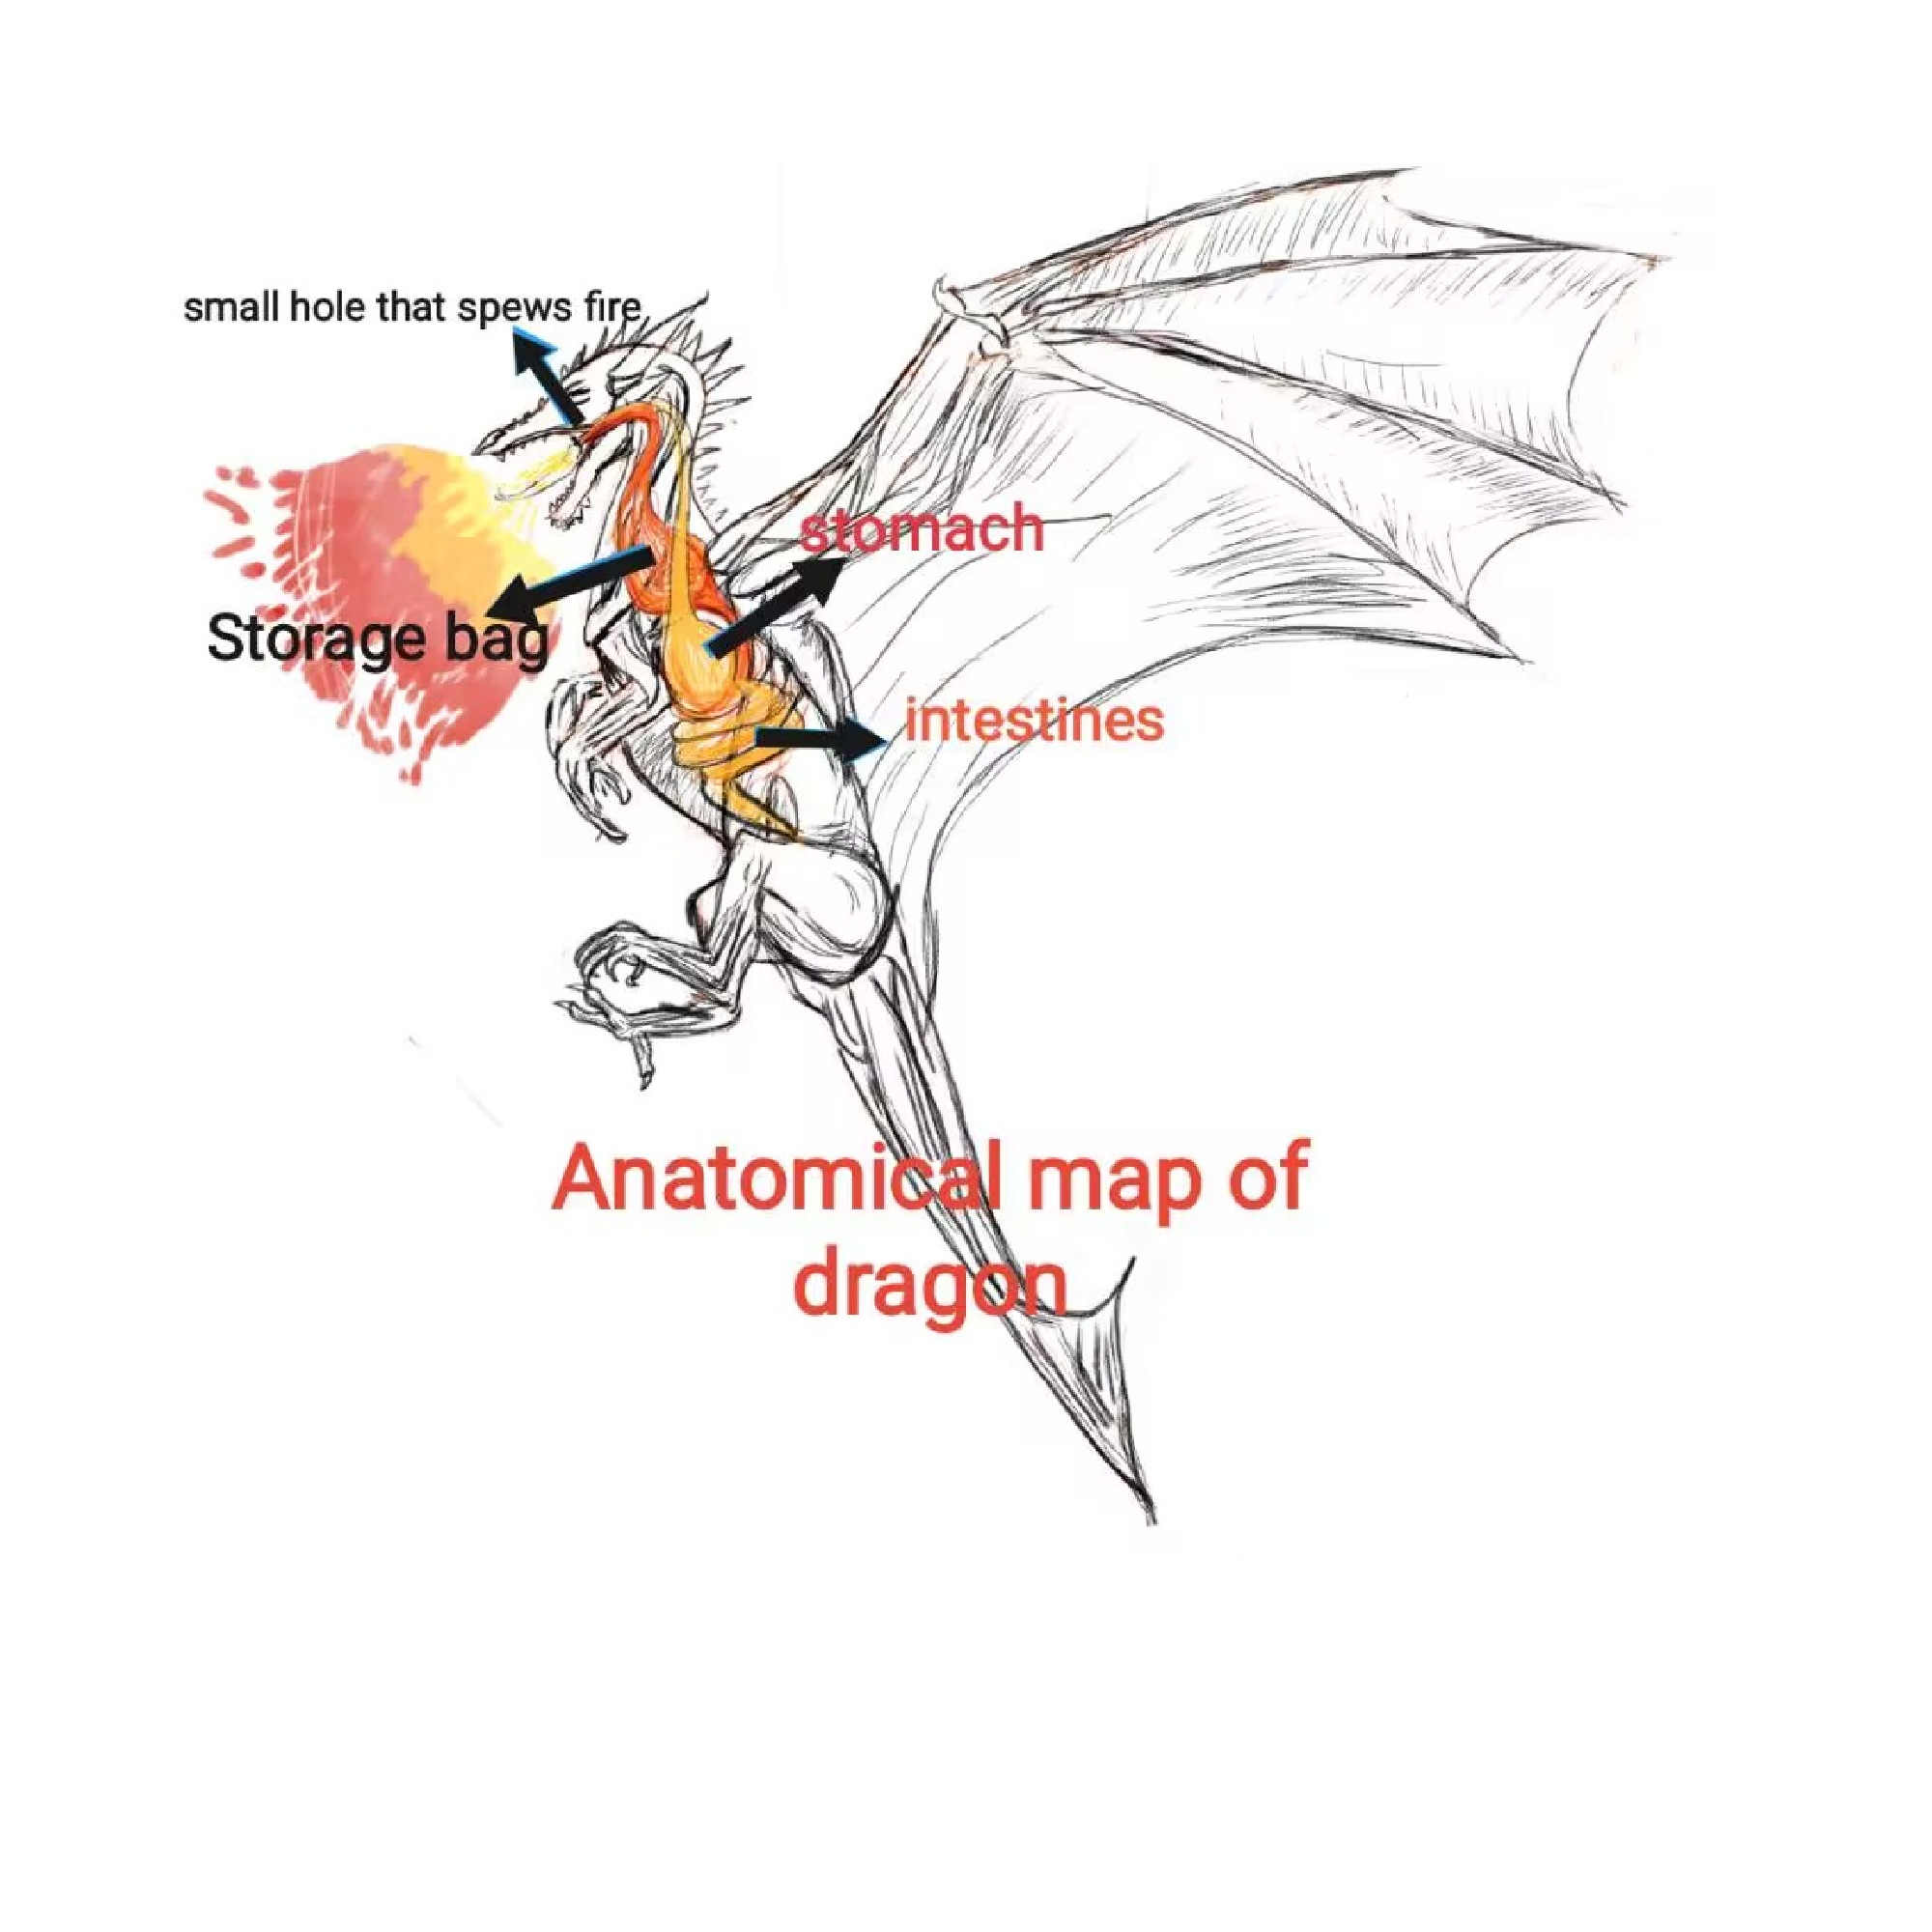
\includegraphics[width=0.5\textwidth]{easymcm/img/spitting fire picture(1).pdf}
	\caption{Spitting fire}\label{fig:spitting fire}
\end{figure}
\vspace{-0.3cm}


Especially, at $25 ^{\circ}C$ and $101 kPa$, the heat equation for combustion is portrayed as formula \eqref{eq:eq4}

\begin{shrinkeq}{-1ex}
	\begin{equation}
    \label{eq:eq4}
	   C_2H_5OH(l) + 3O_2(g) \rightarrow 2CO_2(g) + 3H_2O(l) \quad \Delta H = -1366.8 KJ/mol
	\end{equation}
\end{shrinkeq}

Ethanol releases energy in this reaction process. We assume that the dragon burns $0.1\%$  of its body weight per day, then the energy consumption of burning ethanol per day is $(29.7\cdot W) kJ$. To simplify our model, the energy used by compressing it to its ignition point can be ignored, considering the fact that the ignition point of ethanol is relatively low when compared with most liquids that can be employed to ignite the fire.

\subsection{Resting metabolism model}
For a more precise evaluation of energy consumption for survival in dragons, we will examine the resting metabolic rate independently. By reading the literature, we have learned that the metabolic rate of a living organism is positively proportional to the $\frac{3}{4}$ power of its weight, which can be represented by equation \eqref{eq:eq5}.

\begin{shrinkeq}{-1ex}
	\begin{equation}
    \label{eq:eq5}
	   V_a = BW ^{\frac{3}{4}}
	\end{equation}
\end{shrinkeq}

 Then we take temperature into consideration, and equation\eqref{eq:eq5} changes into the below equation:
\begin{shrinkeq}{-1ex}
	\begin{equation}
    \label{eq:eq6}
	   V_a = BW ^{\frac{3}{4}} * f(T)
	\end{equation}
\end{shrinkeq}

In equation \eqref{eq:eq6}, $V_a$ means energy consumption for resting metabolism per day ,while $W$ is weight. $B$ is the coefficient to connect $V_a$ and $W^\frac{3}{4}$. $f(T)$ is the influence of temperature. We use the lizard's resting metabolic rate to fit our model, and we get $B = 2929.4 kJ/kg$, $f(T) = 0.03T + 0.1$.

\subsection{Dragon's flight model}
The lift $L$ and drag $D$ forces are expressed in terms of lift and drag coefficients $CL$ and $CD$, respectively, wing area $S$ and air speed $V$ by the familiar equations: 

\begin{shrinkeq}{-1ex}
	\begin{equation}
    \label{eq:eq7}
	  L = 0.5\rho SV^2CL 
	\end{equation}
\end{shrinkeq}
\vspace{-0.2 cm}
\begin{shrinkeq}{-1ex}
	\begin{equation}
    \label{eq:eq8}
	   D = 0.5\rho SV^2CD = 0.5\rho SV^2(CD_i + CD_0)
	\end{equation}
\end{shrinkeq}

where $\rho$ is air density, and $CD_i$ and $CD_0$ represent the induced 
and friction components of drag, respectively. $CD_0$ is approximately constant (but see below). The key prediction of lifting-line theory (e.g. Prandtl and Tietjens, 1934) is that: 

\begin{shrinkeq}{-1ex}
	\begin{equation}
    \label{eq:eq9}
	   CD_i \propto CL^2
	\end{equation}
\end{shrinkeq}
This is the equation of the so-called ‘lift polar’, and it is this that determines the shape of the power curve. In steady-level flight with a fixed wing, lift balances weight $Mg$, where $M$ is mass and $g$ is the acceleration due to gravity, and the thrust $T$ applied must equal the drag $D$. The mechanical power output $Pmech$ is then given by: 
\begin{figure}[h]
	\centering
	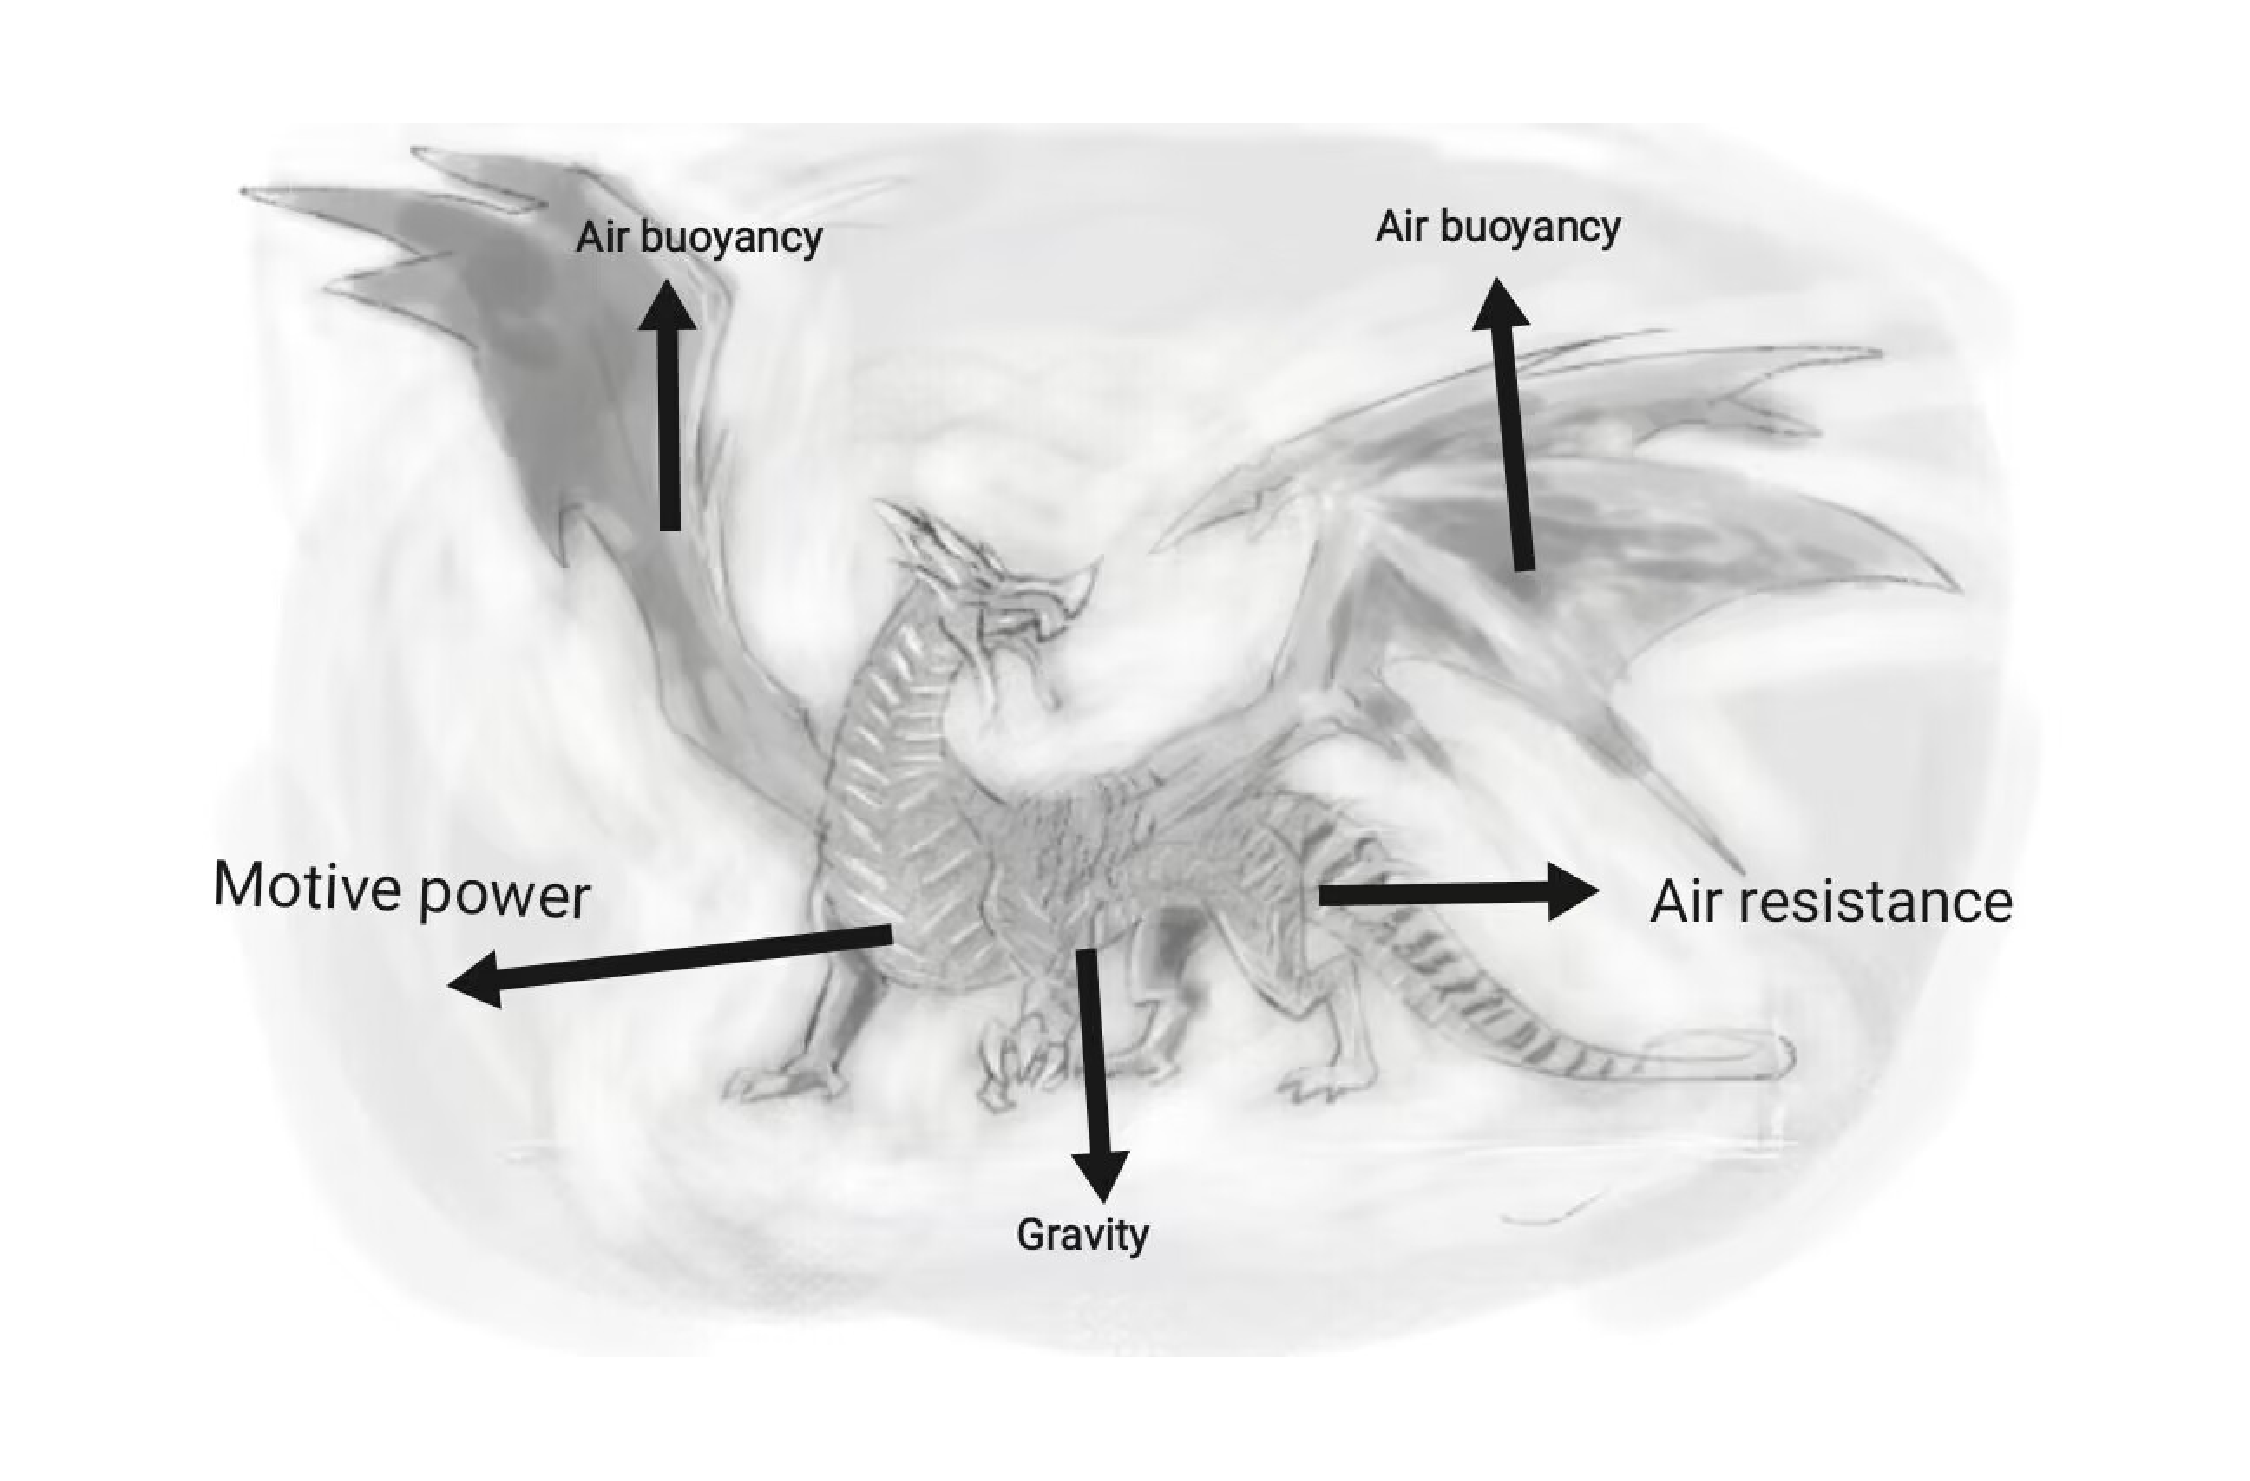
\includegraphics[width=0.7\textwidth]{easymcm/img/ab.pdf}
	\caption{Force analysis of dragon in flight
}
\end{figure}
\begin{shrinkeq}{-1ex}
	\begin{equation}
    \label{eq:eq10}
	   Pmech = TV = DV = \frac{\alpha}{V} + \beta V^3
	\end{equation}
\end{shrinkeq}

According to aerodynamics, the speed $v$ required for a dragon to maintain lift-to-weight balance while flying at a steady level is related to its weight $W$ and wing surface area $A$. The connection can be described as equation \eqref{eq:eq11}
\begin{shrinkeq}{-1ex}
	\begin{equation}
    \label{eq:eq11}
	   v = \sqrt{\frac{2Wg}{CL\rho A}}
	\end{equation}
\end{shrinkeq}

$g$ is the acceleration of gravity, $CL$ is the lift coefficient, which is close to 1 for a normal shape; $\rho$ is the air density. For a given body shape of the dragon, $W$ is proportional to the cube of the length or wingspan, $A$ is proportional to the square of the length or wingspan, and $CL$ is typically close to 1. It can be seen that the velocity $v$ required for level flight is proportional to the $\frac{1}{6}$ power of the weight $W$. At the same time, once ignoring the lifting airflow, the resistance $F$ encountered when flying in the air is associated with the velocity $v$ and the projected area $B$ of the body as follows:
\begin{shrinkeq}{-1ex}
	\begin{equation}
    \label{eq:eq12}
	   F = CD\rho Bv^2
	\end{equation}
\end{shrinkeq}

$CD$ is the drag coefficient, which is typically close to 0.1 for streamlined objects; $\rho$ is the air density.

The power $P$ required for flapping flight is $P=F*v$, $P$ is proportional to the cube of velocity $v$ and the frontal area $B$. For a given body shape of the dragon, $B$ is proportional to the square of its length or wingspan. It can be seen that the power $P$ required for level flight is proportional to the $\frac{7}{6}$ power of $W$.That is:
\begin{shrinkeq}{-1ex}
	\begin{equation}
    \label{eq:eq13}
	   P = Pmech W^{\frac{7}{6}}
	\end{equation}
\end{shrinkeq}
Then we consider that the larger the dragon, the stronger the gliding ability, so the above equation should be modified as:
\begin{shrinkeq}{-1ex}
	\begin{equation}
    \label{eq:eq13}
	   P = Pmech W^{\frac{3}{4}}
	\end{equation}
\end{shrinkeq}

\subsection{Total metabolism of dragon}
\begin{figure}[h]
	\centering
	\begin{minipage}[t]{0.45\textwidth}
		\centering
		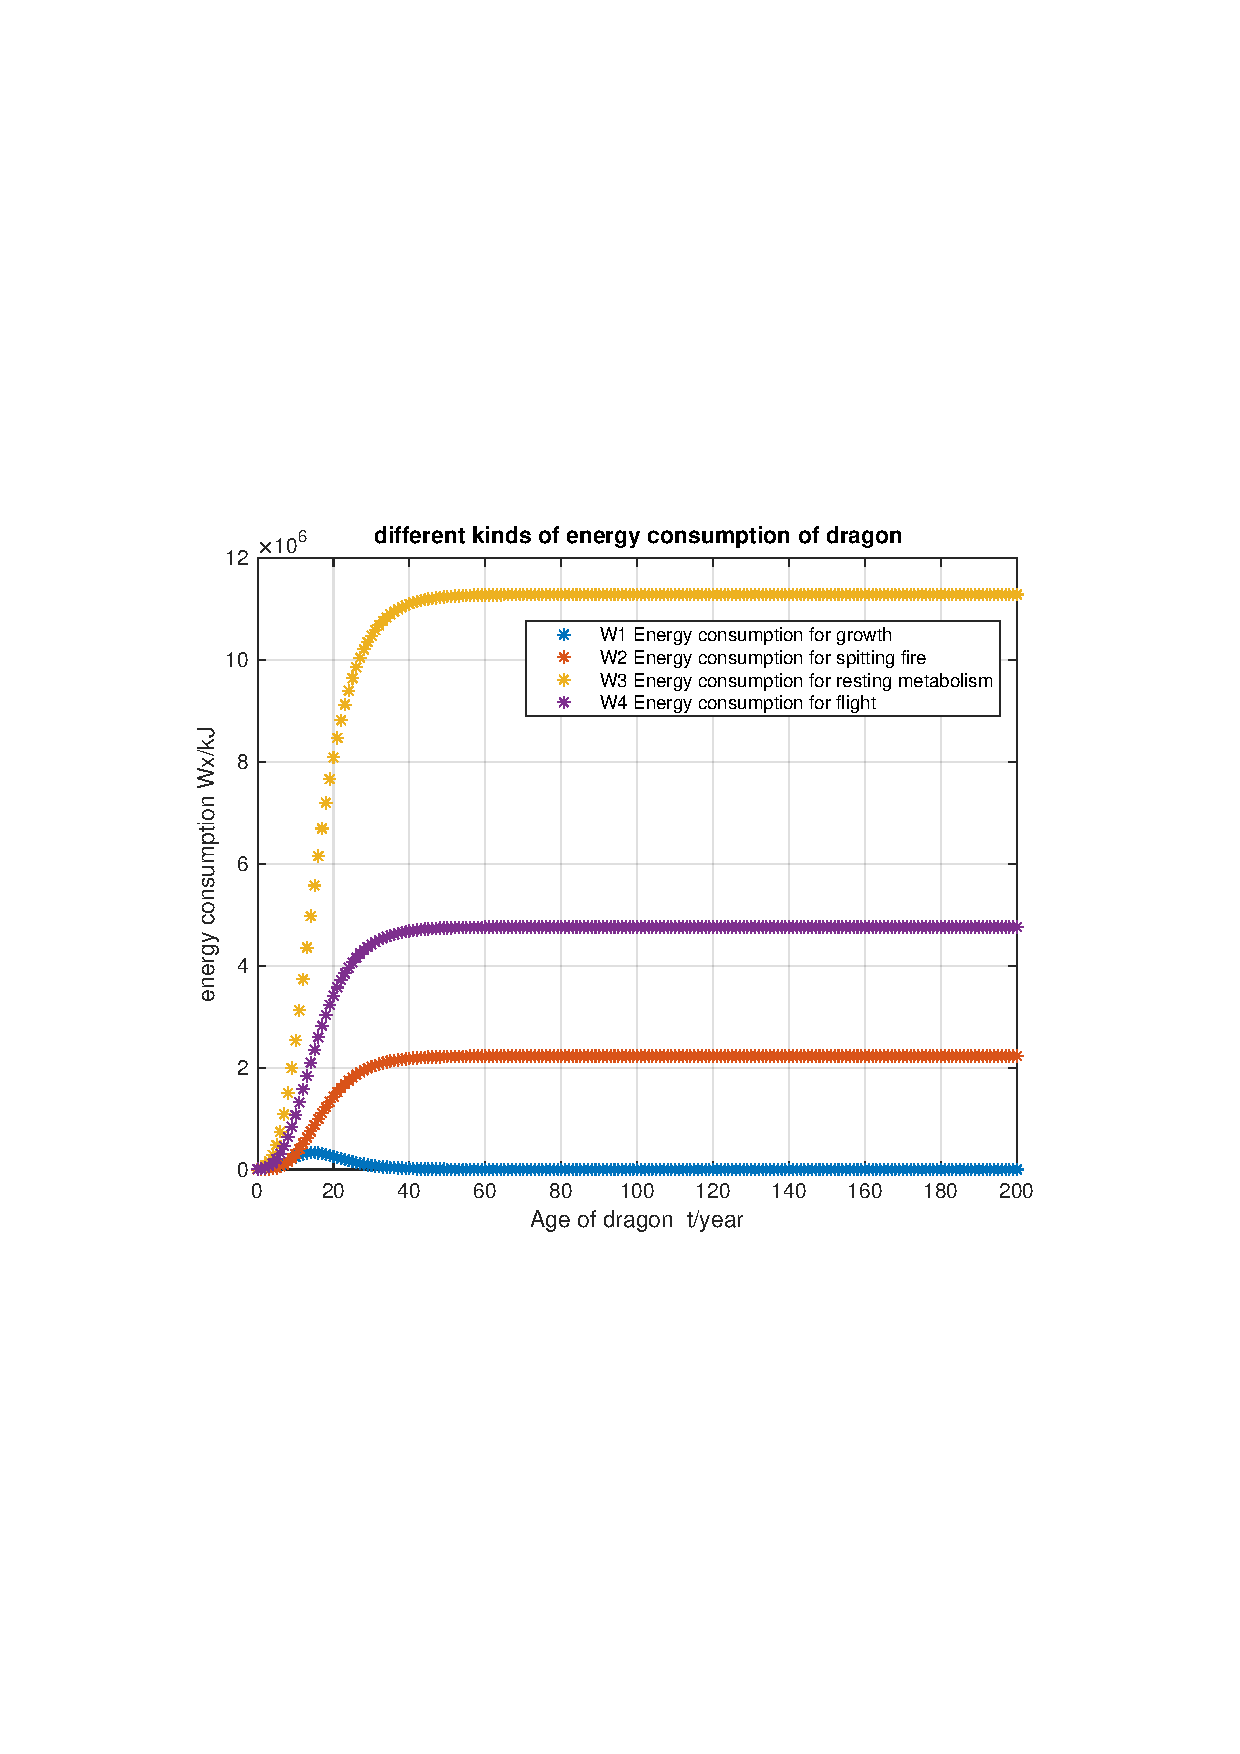
\includegraphics[width=1\textwidth]{easymcm/img/different kinds of energy consumption of dragon.pdf}
		\caption{different kinds of energy consumption }
	\end{minipage}
	\begin{minipage}[t]{0.45\textwidth}
		\centering
		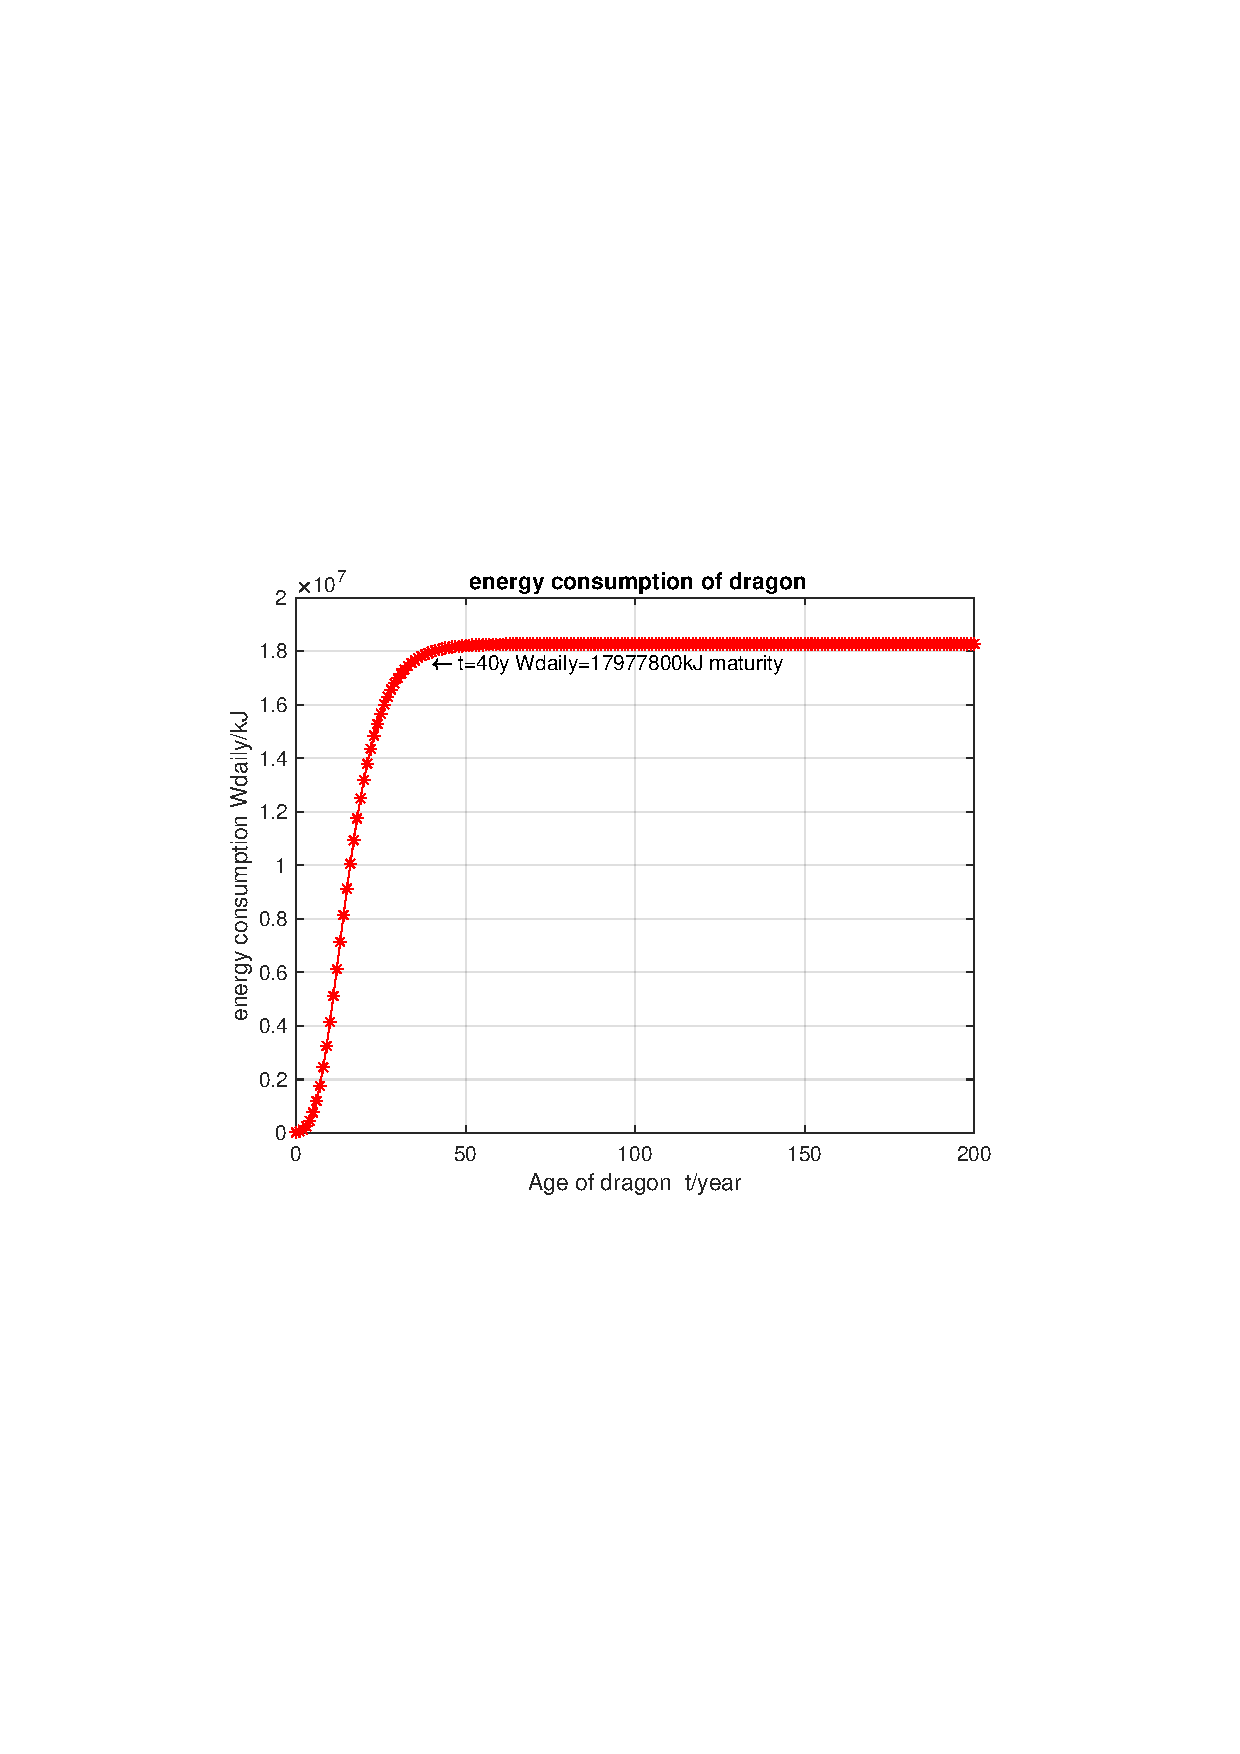
\includegraphics[width=1.05\textwidth]{easymcm/img/energy consumption of dragon.pdf}
		\caption{energy consumption of dragon}
	\end{minipage}
\end{figure}
Finally, we get the total metabolism of the dragon, which is:
\begin{shrinkeq}{-1ex}
	\begin{equation}
    \label{eq:eq14}
	   W_{daily} = W1+W2+W3+W4
	\end{equation}
\end{shrinkeq}
\begin{shrinkeq}{-1ex}
	\begin{equation}
    \label{eq:eq14}
	   W1 = k*ln(\frac{W_\infty}{W_0})W exp(-kt)*\frac{G}{365}
	\end{equation}
\end{shrinkeq}
\begin{shrinkeq}{-1ex}
	\begin{equation}
    \label{eq:eq14}
	   W2 = 29.7W
	\end{equation}
\end{shrinkeq}
\begin{shrinkeq}{-1ex}
	\begin{equation}
    \label{eq:eq14}
	   W3 = BW^{\frac{3}{4}}*(0.03T+0.1) 
	\end{equation}
\end{shrinkeq}
\begin{shrinkeq}{-1ex}
	\begin{equation}
    \label{eq:eq14}
	   W4 = (\frac{\alpha}{V} + \beta V^3)W^\frac{3}{4}
	\end{equation}
\end{shrinkeq}




\section{Model \uppercase\expandafter{\romannumeral2} : Pasture growth model }
\vspace{-0.3cm}
\subsection{Model overview}
In our previous work, we acquired the energy supply needed to domesticate three dragons. We demarcated pasture areas for the dragons and used them for livestock (mainly sheep). The growth of forage was modeled mathematically according to the predator-prey model. Direct factors affecting the growth of herbage include sunlight, moisture, temperature, etc., as well as indirect factors such as the energy acquisition coefficient of sheep and the predation coefficient of dragons. Considering the authenticity of the model, we added a retarded growth term on the basis of the original model, so as to maintain a dynamic balance between the forage and the number of sheep. Finally, we selected three grasslands with different temperature zones in reality and brought them into the model for verification to ensure the robustness the model. 
\begin{figure}[h]
	\centering
	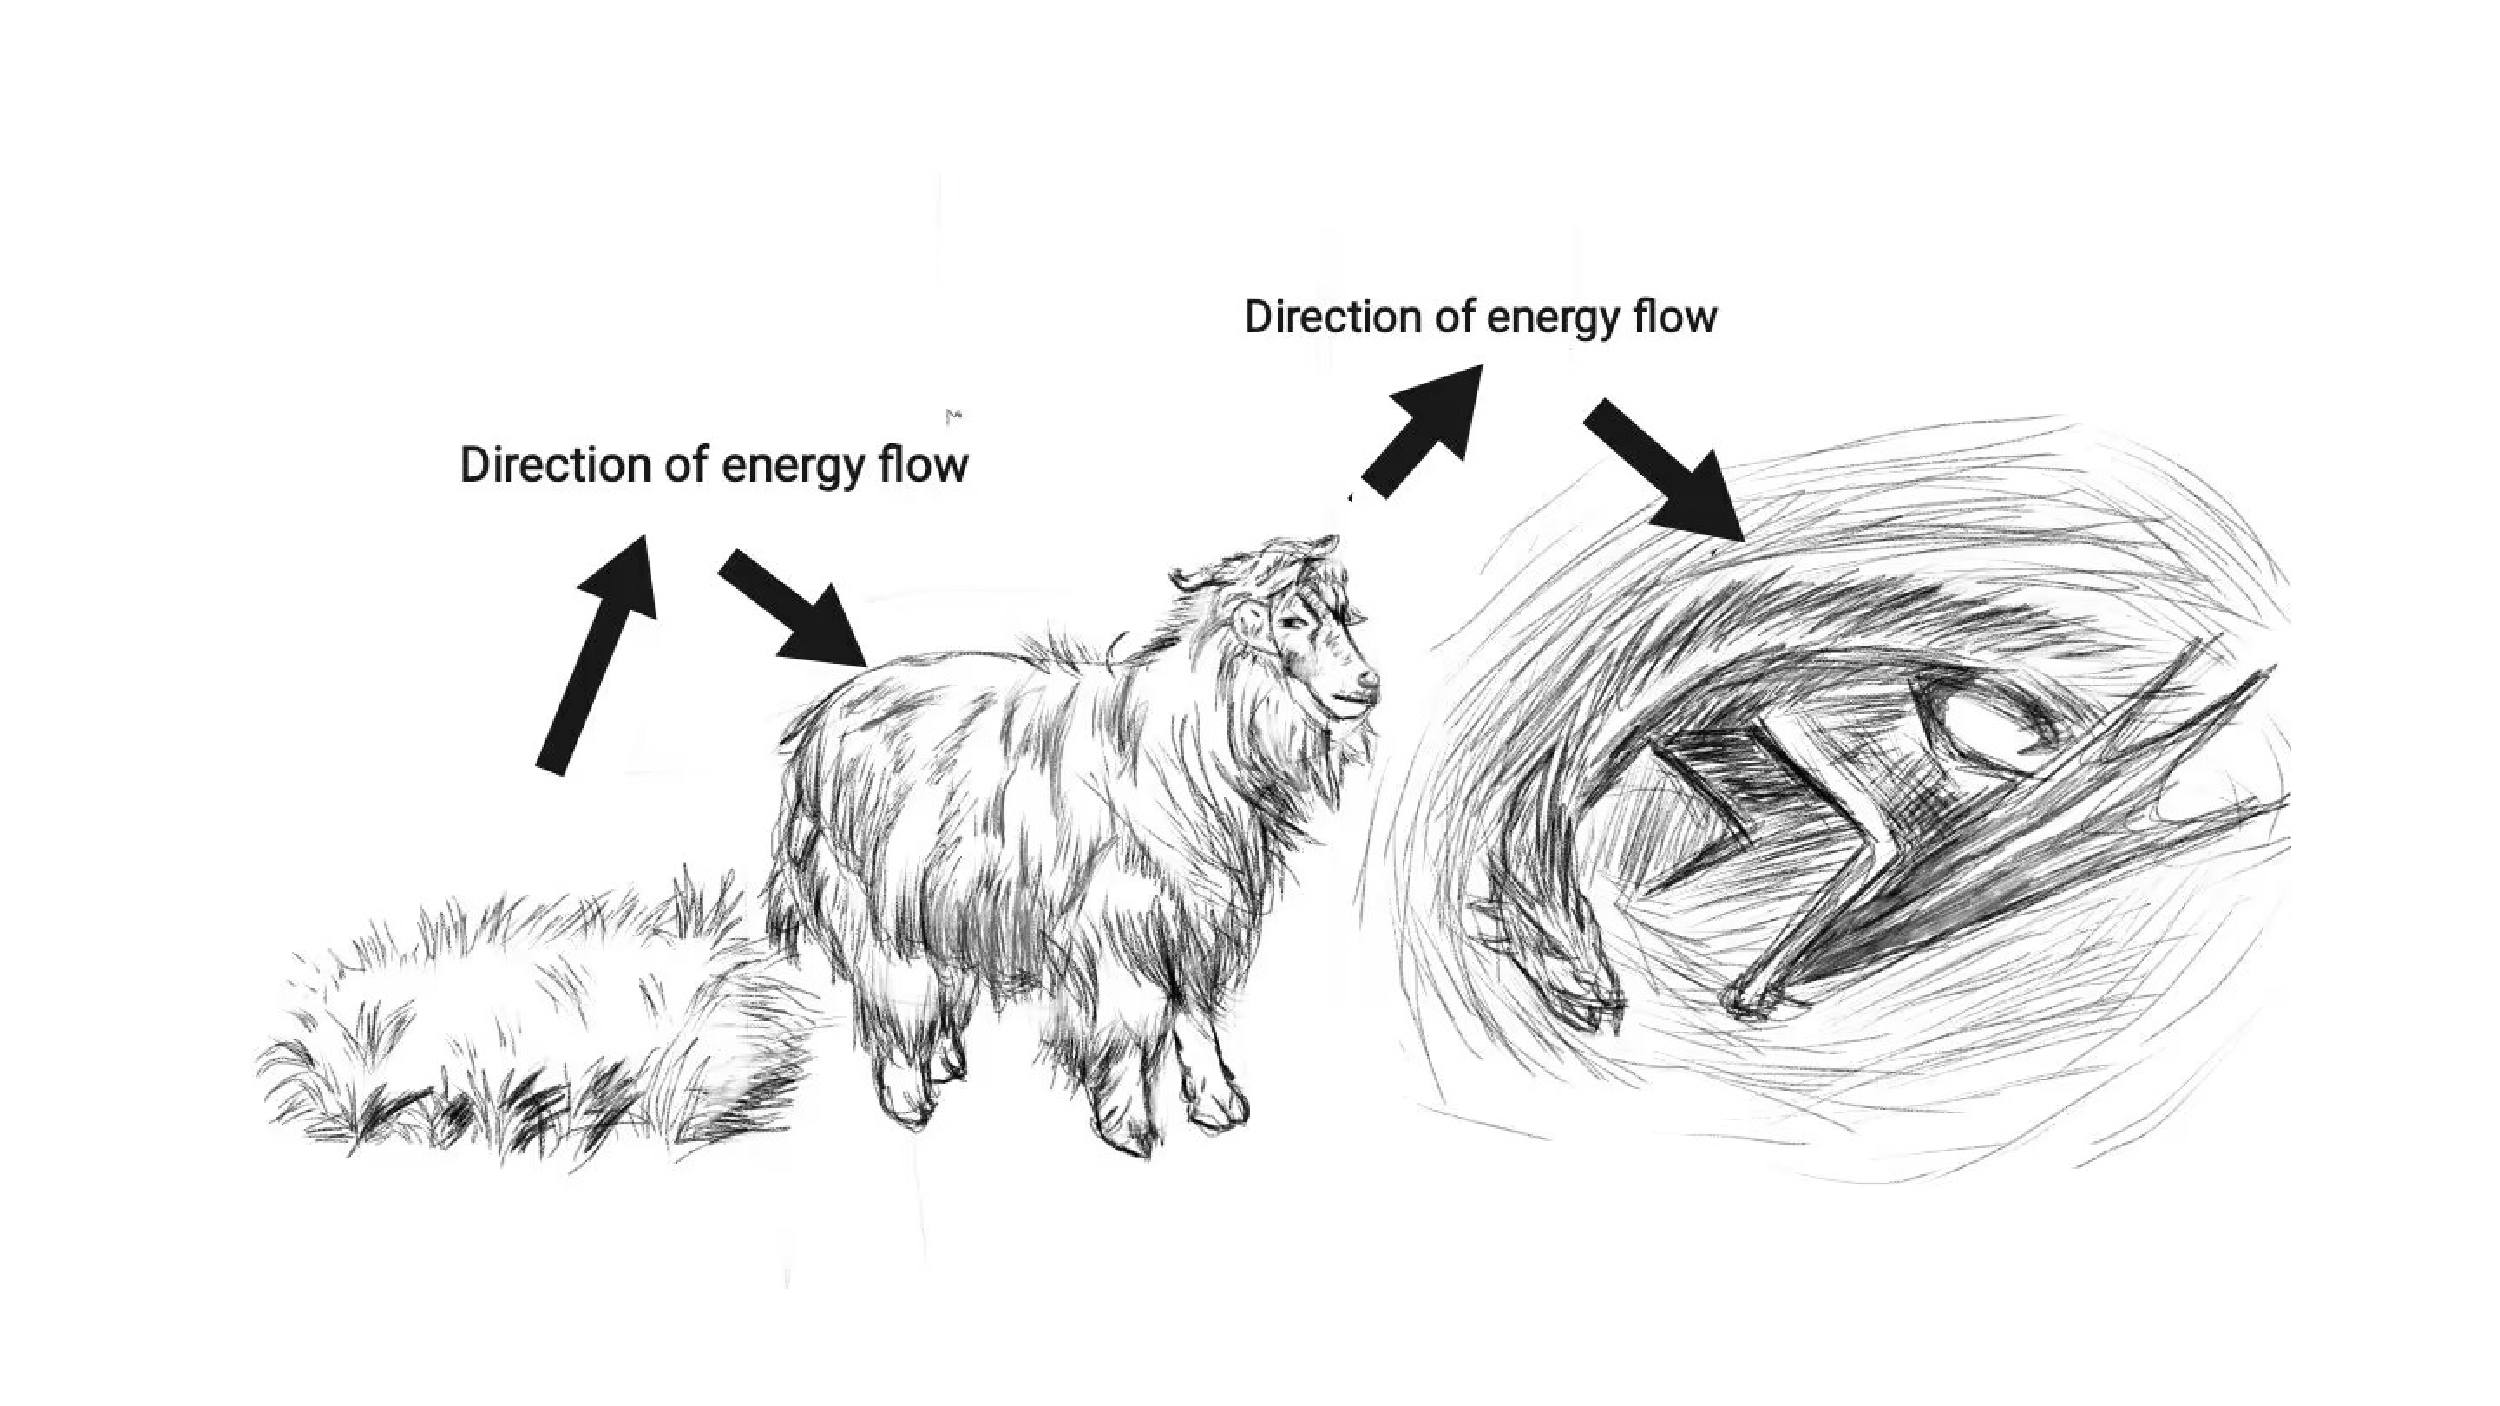
\includegraphics[width=0.8\textwidth]{easymcm/img/abc.pdf}
	\caption{Direction of energy flow}
\end{figure}
\subsection{Predator Prey model}
The variation of prey population x(t) and predator population y(t) over time is given by the following Predator Prey equation:
\begin{shrinkeq}{-1ex}
	\begin{equation}
    \label{eq:eq16}
	\dot{x}(t)=x(r-a y)=r x-a x y 
	\end{equation}
\end{shrinkeq}
\begin{shrinkeq}{-1ex}
	\begin{equation}
    \label{eq:eq17}
	\dot{y}(i)=y(-d+b x)=-d y+b x y
	\end{equation}
\end{shrinkeq}

The first term on the right side of the equation shows the tendency of the groups themselves to change in their natural environment, while the second term describes the changes caused by prey being killed by predators. In our study, the prey was pasture, whose population was represented by area, and the predator was sheep. 
Specifically, you can think of r as the natural growth rate of prey, the difference between their natural birth rate and their natural death rate. It is assumed that the prey will always have sufficient resources to survive, and that if there are no natural predators, the population will continue to grow exponentially. And for predators, if they don't have prey, they starve to death for lack of food resources, and the natural growth rate is negative, so d in this equation can be thought of as their natural mortality rate. 

 $\alpha$ can be seen as the proportion of prey captured by the predator per unit time, so the total number of prey captured in the $dt$ interval is $\alpha$*$dt$*$x$*$y$, which corresponds to the second term on the right side of the equation. When predators have food to fill their stomachs, they have a chance to reproduce. There's a conversion between the number of prey caught and the number of baby predators born, and the factor $b$ that appears in the equation is such a conversion factor. 

Interestingly, although these differential equations are nonlinear and have no analytical solutions that can be expressed in terms of elementary trigonometric functions, their solutions are regularly periodic. As Alfred J. Lotka himself wrote in a 1920 paper: It was, therefore, with considerable surprise that the writer, on applying his method to certain special cases, found these to lead to undamped, and hence indefinitely continued, oscillations.

\begin{figure}[htbp]
	\centering
	\begin{minipage}[t]{0.45\textwidth}
		\centering
		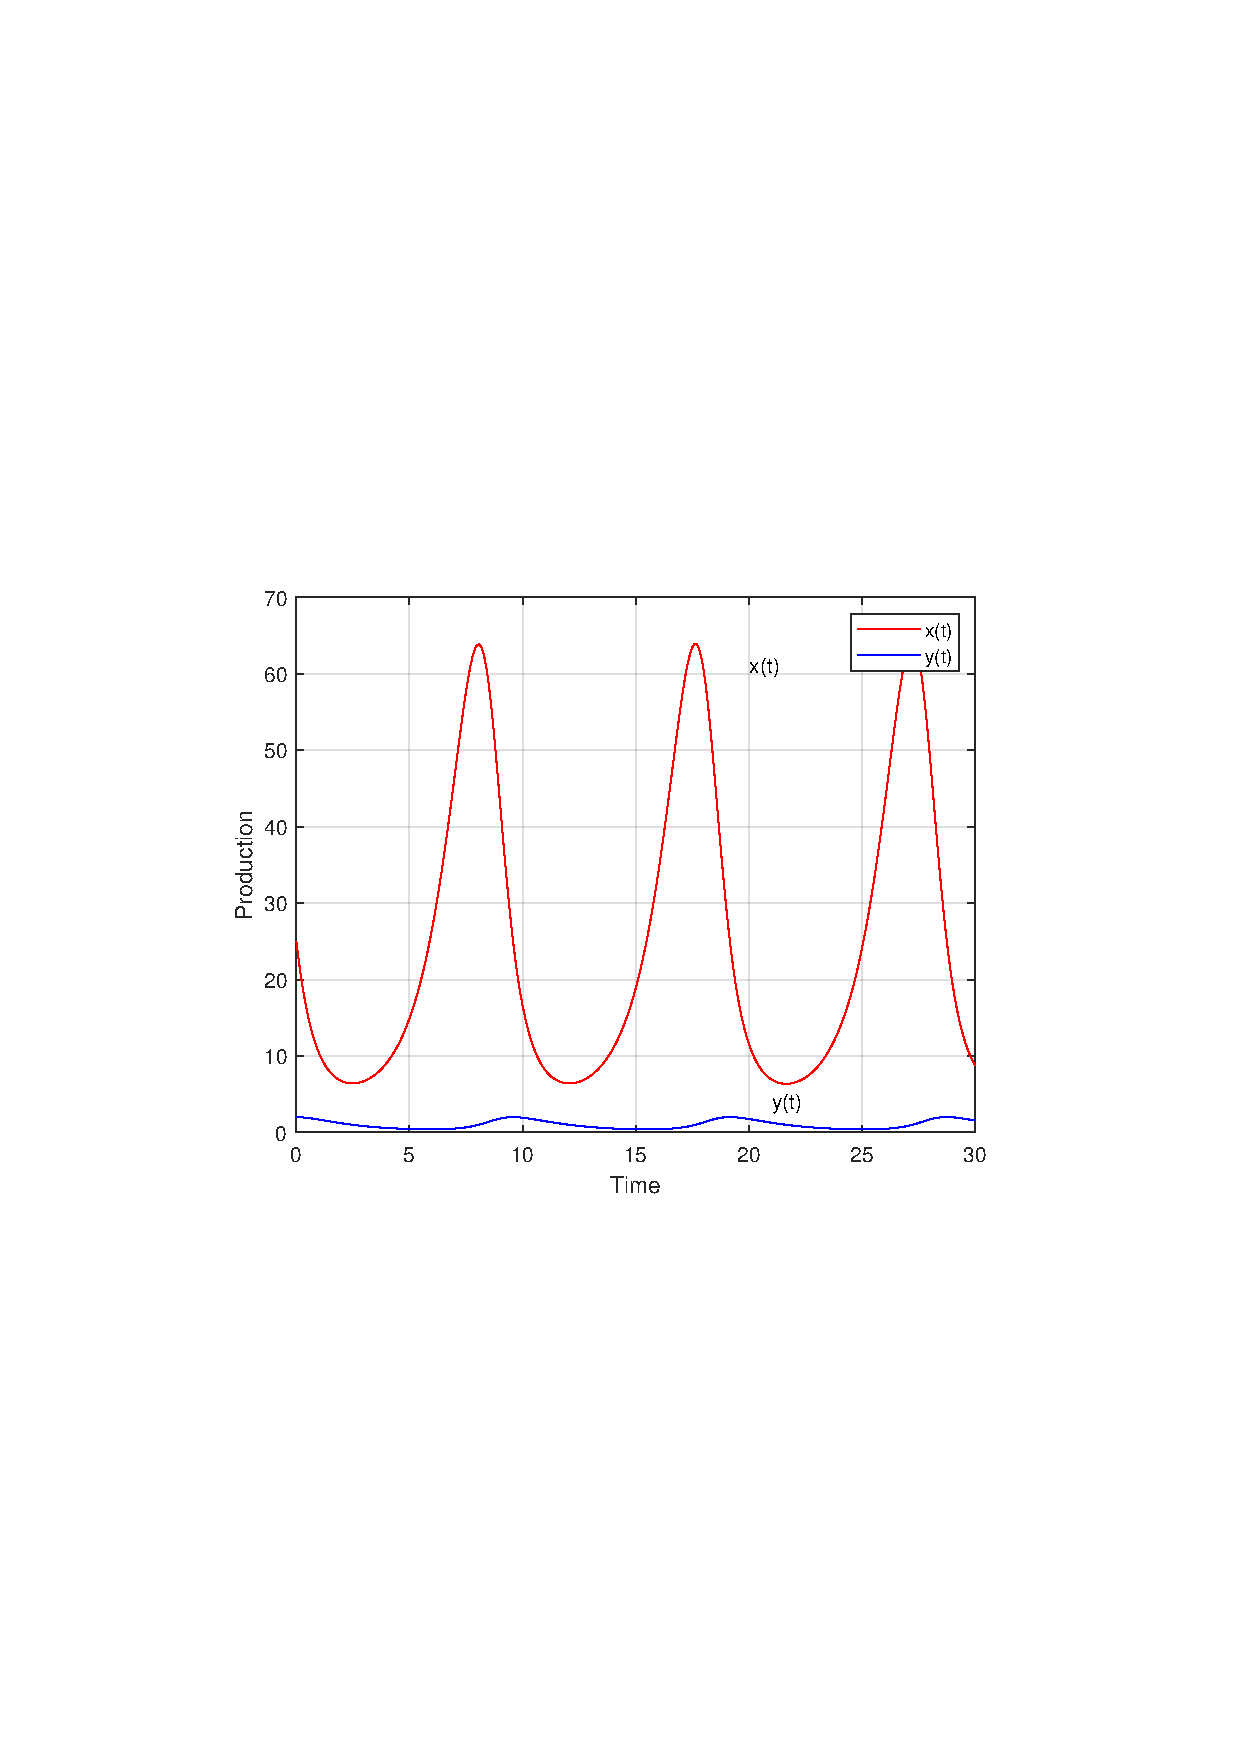
\includegraphics[width=1\textwidth]{Predator_Prey_model.pdf}
		\caption{Predator Prey model}
        % \label{fig:quanju}
	\end{minipage}
	\begin{minipage}[t]{0.45\textwidth}
		\centering
		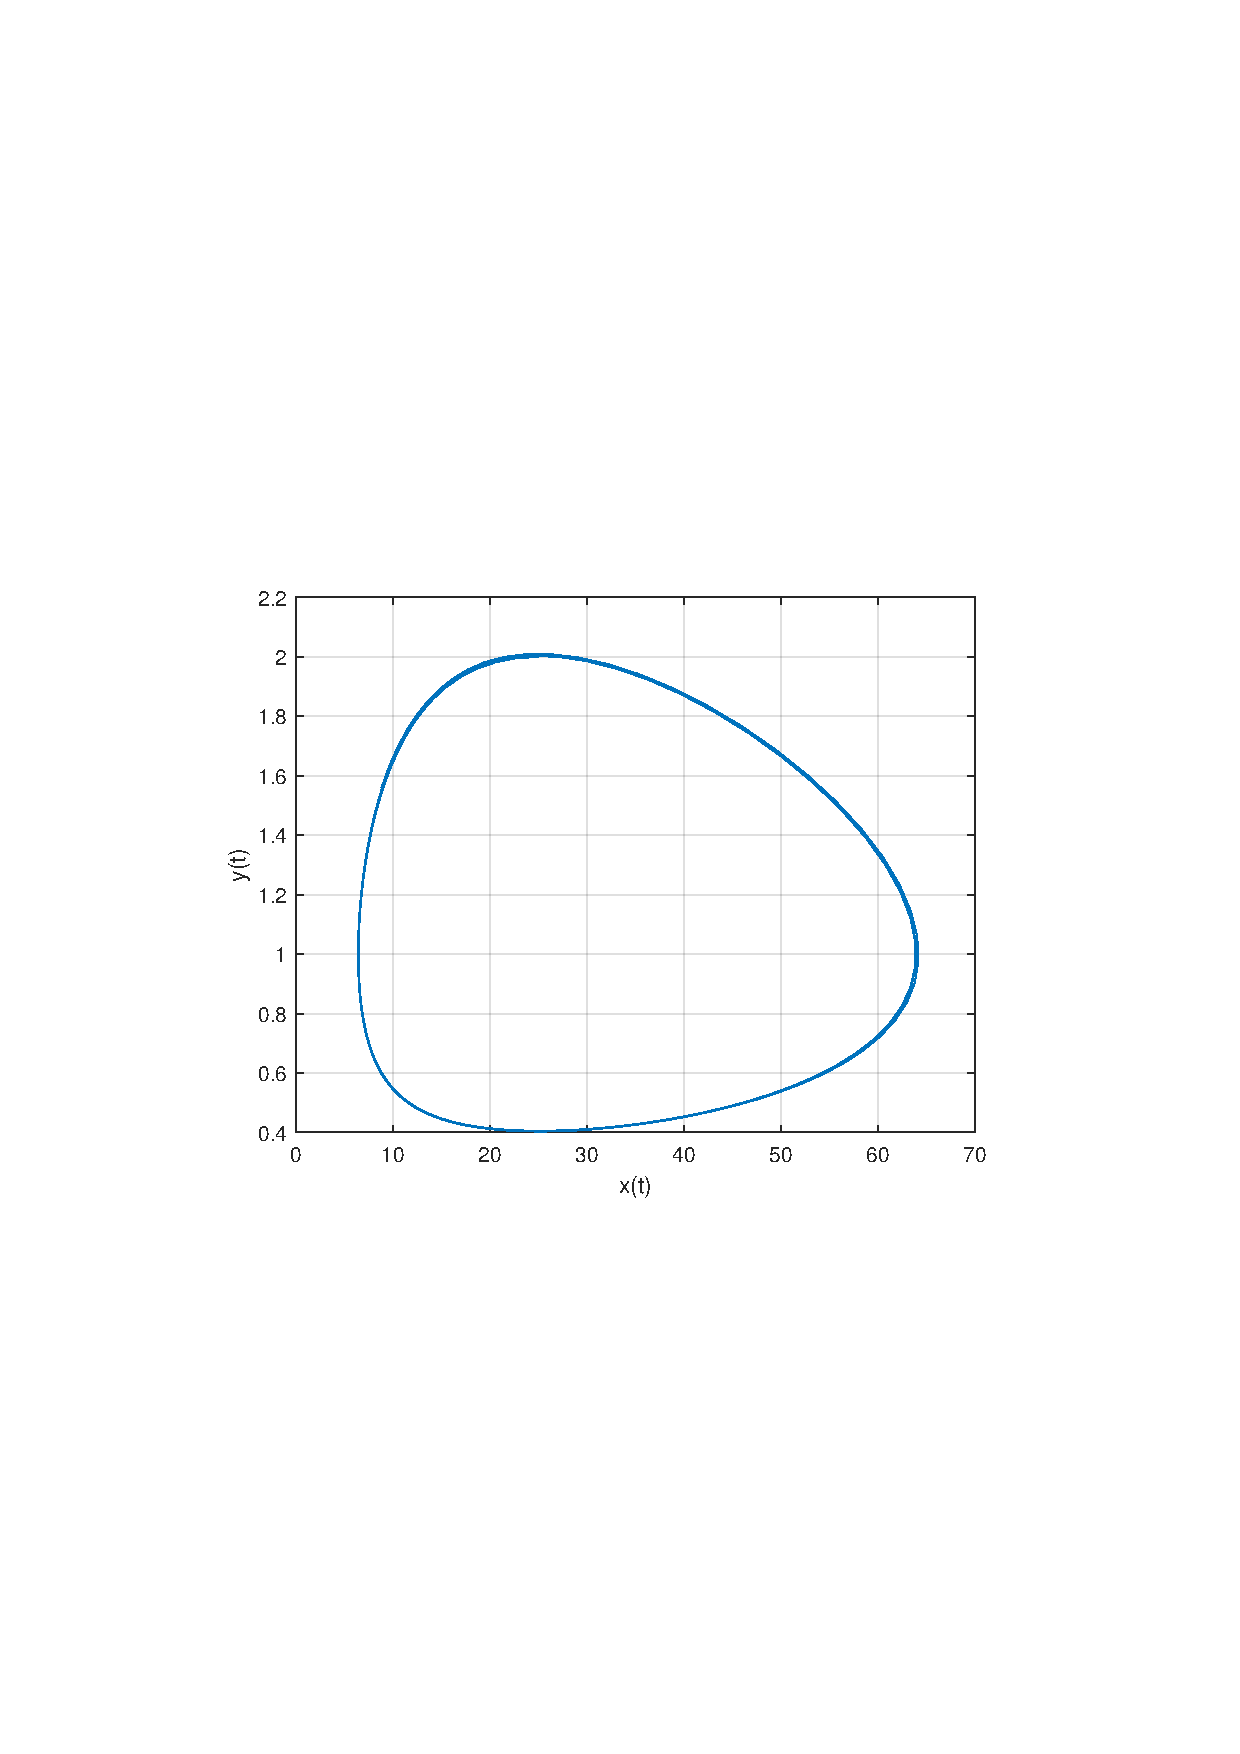
\includegraphics[width=0.98\textwidth]{phase_trajectory1.pdf}
		\caption{phase trajectory}
        % \label{fig:jubu}
	\end{minipage}
\end{figure}

In the figure, we can clearly see that the pasture and sheep numbers show undamped oscillation. And in the phase orbit diagram, there is also a closed curve, which indicates that the quantity of the two changes periodicity.

\subsection{logistic Predator Prey model}
Although Volterra model can explain some phenomena, it is bound to have many limitations as a mathematical model that almost reflects the real object.

First, according to literature [x], most predator-prey systems do not observe the periodic oscillations shown in Volterra's model, but tend to some equilibrium state, i.e. there is a stable equilibrium point. In fact, if the logistic term for self-retardation is added to Volterra's model, The final dynamic equilibrium state can be simulated. 

Secondly, according to literature [y], the long-term ecological balance system with periodic changes in nature should be structurally stable, that is, after the system deviates from the original periodic orbit due to inevitable interference, its internal restriction will make the system restore to the original, such as the recovery period and amplitude. The Volterra model describes periodic states that are not structurally stable. Therefore, we finally chose to add logistic retarders to simulate the herbage - sheep model:

\begin{shrinkeq}{-1ex}
	\begin{equation}
    \label{eq:eq17}
	 \dot{x}_1(t)=r_1 x_1\left(1-\frac{x_1}{N_1}-\sigma_1 \frac{x_2}{N_2}\right)
	\end{equation}
\end{shrinkeq}
\begin{shrinkeq}{-1ex}
	\begin{equation}
    \label{eq:eq18}
	 \dot{x}_2(t)=r_2 x_2\left(-1+\sigma_2 \frac{x_1}{N_1}-\frac{x_2}{N_2}-3m\right)
	\end{equation}
\end{shrinkeq}
\begin{itemize}
\vspace{-0.2cm}
\item[$\bullet$] \textbf{$r_1$ }stands for Grassland growth parameter. 
\vspace{-0.2cm}
\item[$\bullet$] \textbf{$r_2$ }represents Sheep population growth parameters.
\vspace{-0.2cm}
\item[$\bullet$] \textbf{$N_1$ }is Saturated yield of grassland.
\vspace{-0.2cm}
\item[$\bullet$] \textbf{$N_2$ }is Sheep saturation yield (artificially controlled).
\vspace{-0.2cm}
\item[$\bullet$] \textbf{$\sigma_1$ }represents The reverse effect of grass yield on sheep.
\vspace{-0.2cm}
\item[$\bullet$] \textbf{$\sigma_2$ }is Predation coefficient of sheep.
\vspace{-0.2cm}
\item[$\bullet$] \textbf{$m$ }is Predation coefficient of a dragon.
\end{itemize}
\vspace{-0.3cm}

For the dragon, the value of predation rate depends on the energy consumption of the dragon itself, so $m$ is a variable. We plan to judge the value of m according to the two uses of the dragon (war, reproduction and growth), which are quantitatively calculated in the growth model of the dragon.
\begin{figure}[htbp]
	\centering
	\begin{minipage}[t]{0.45\textwidth}
		\centering
		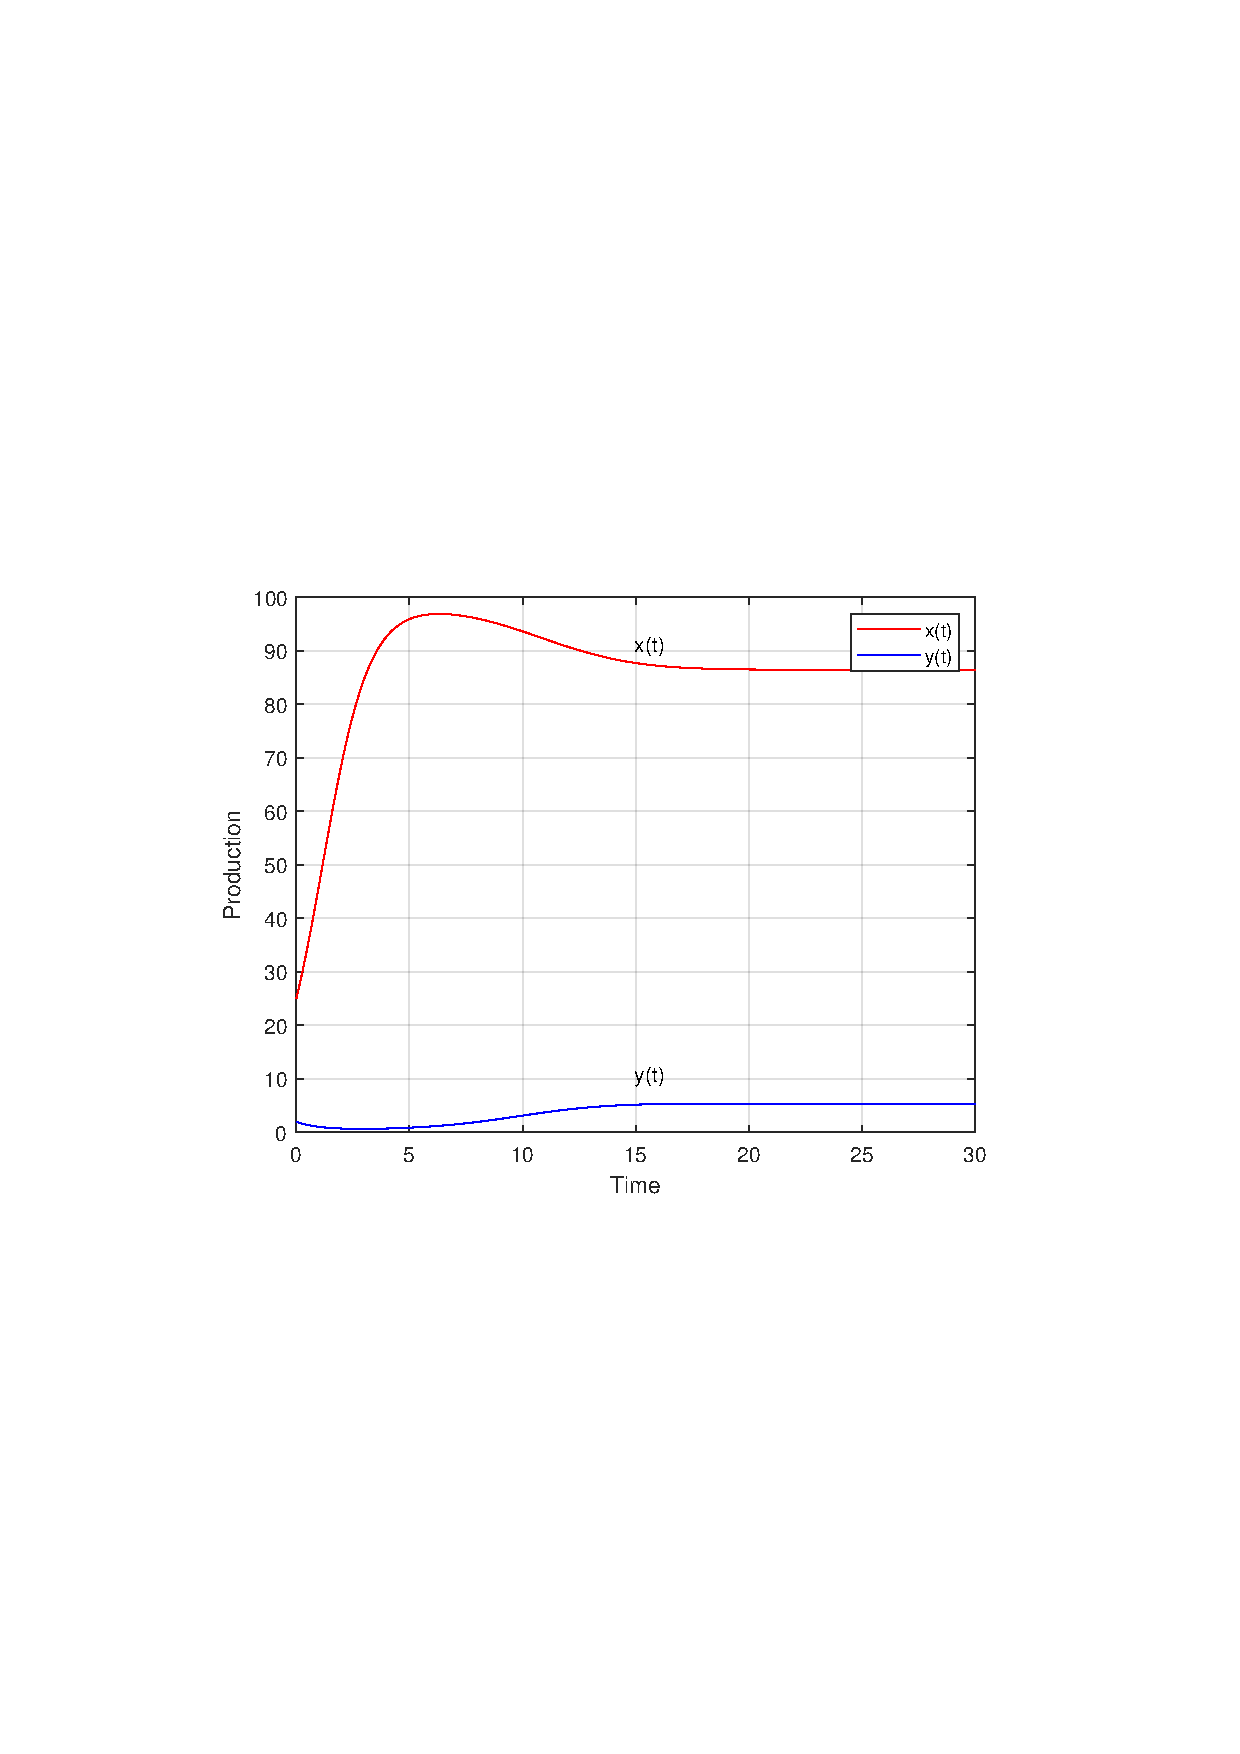
\includegraphics[width=1\textwidth]{logistic_Predator_Prey_model.pdf}
		\caption{logistic Predator Prey model}
        % \label{fig:quanju}
	\end{minipage}
	\begin{minipage}[t]{0.45\textwidth}
		\centering
		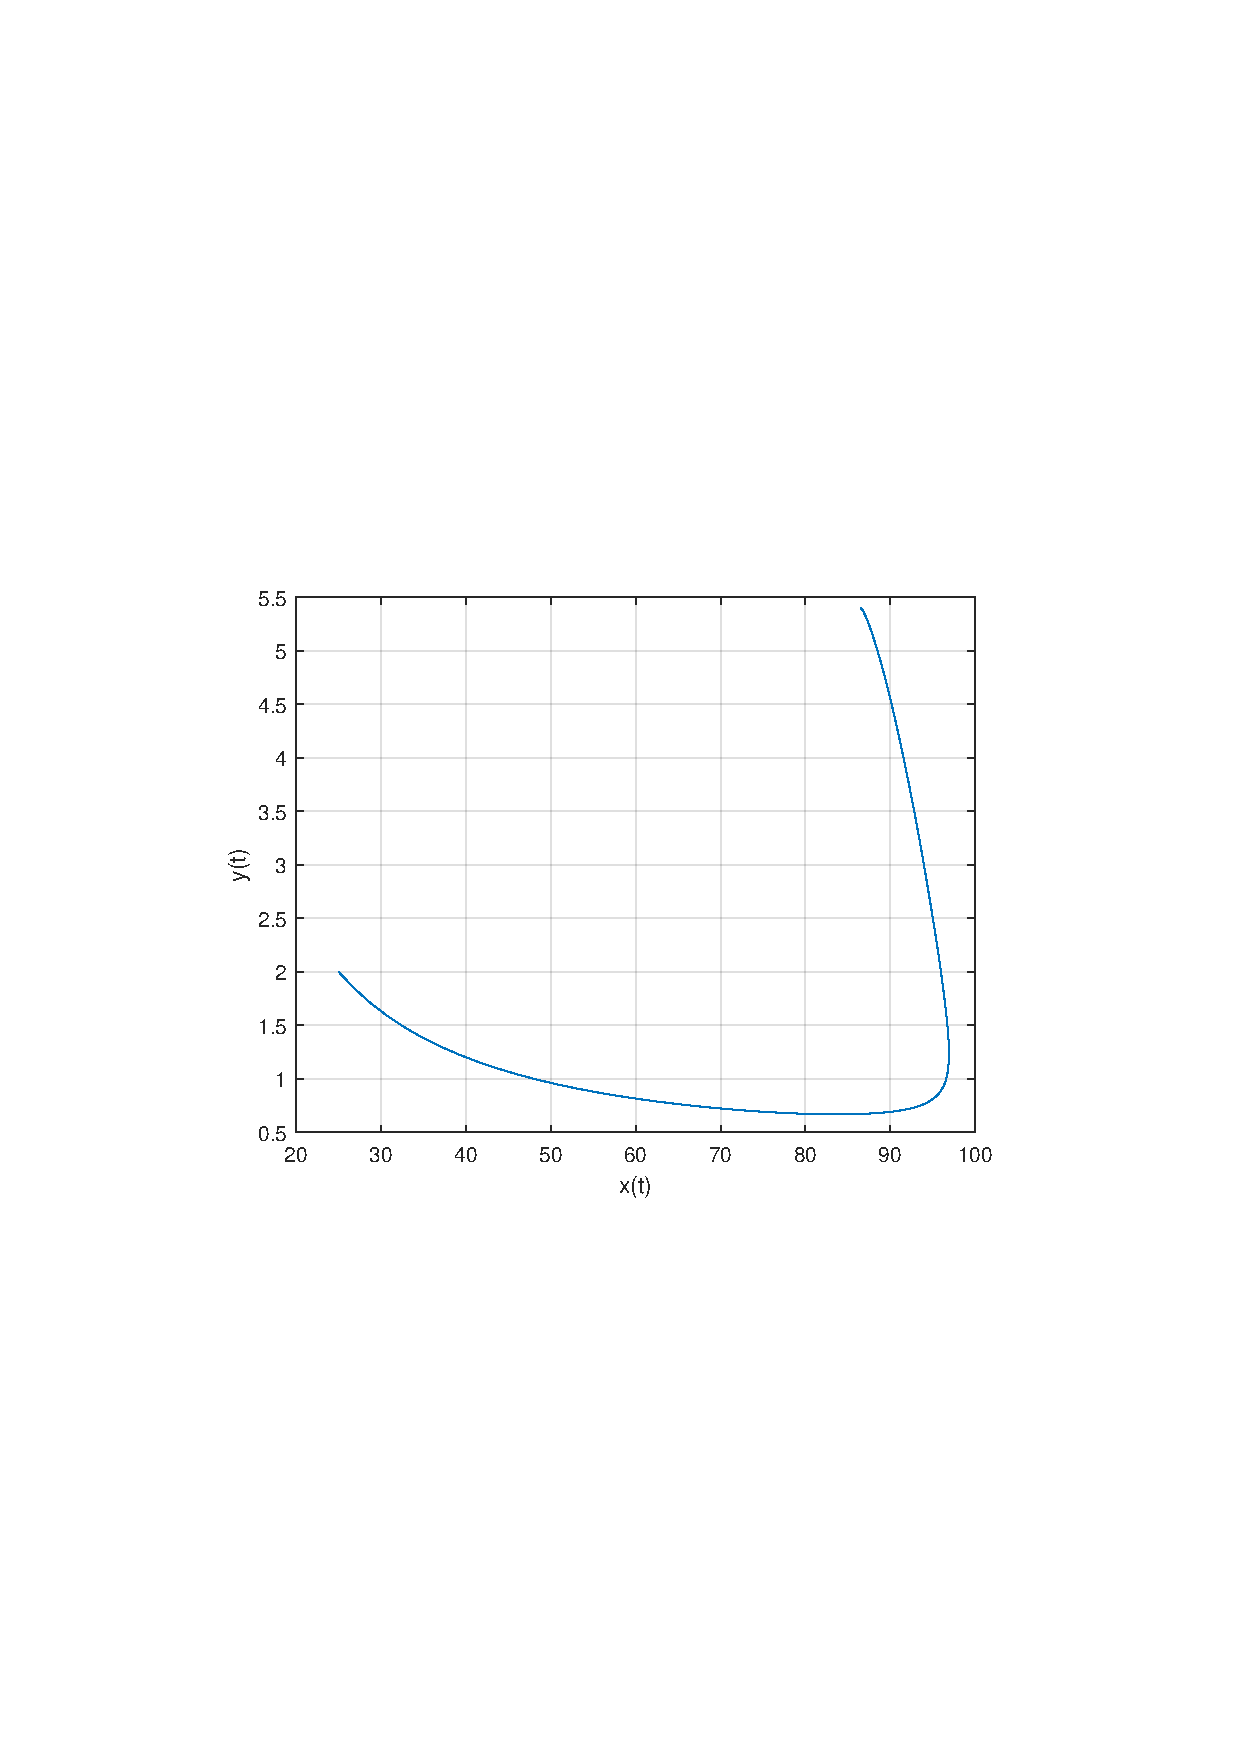
\includegraphics[width=0.98\textwidth]{phase_trajectory2.pdf}
		\caption{phase trajectory}
        % \label{fig:jubu}
	\end{minipage}
\end{figure}

After adding the logistic term, compared with the previous two figures, we can see that after a small fluctuation, the number of sheep and pasture tends to be in dynamic balance. And the phase orbit diagram is no longer a closed curve.
\newpage
\subsection{Grassland net productivity model}
According to the net grassland productivity (NPP) proposed in literature [k], the growth rate r in the formula is closely related to NPP, namely:
\begin{shrinkeq}{-1ex}
	\begin{equation}
    \label{eq:eq20}
	\operatorname{NPP}(x, t)= \operatorname{FAPAR}(x, t) \times \varepsilon_{\max }(x, t) \times 
	T_{\varepsilon 1}(x, t) \times T_{\varepsilon 2}(x, t) \times W_{\varepsilon}(x, t)
	\end{equation}
\end{shrinkeq}

$FAPAR$ is the photosynthetic active radiation absorbed by vegetation, $\varepsilon_{max}$ is the maximum utilization of light energy, $T_{\varepsilon1}$ and $T_{\varepsilon2}$ are temperature stress coefficients, and $W_{\varepsilon}$ is water stress coefficients.

It can be concluded that the grassland growth rate is directly related to the three factors of light, temperature and humidity, which also provides guidance for our future application of the model.

\subsection{Climate - dependent pasture model}
To test the pasture-sheep model, we selected pastureland in three different areas of the real world. They come from the arid region, the warm temperate region and the arctic region. We have obtained the temperature, humidity and light information of these grasslands from relevant websites.

Different temperature zones have different climate characteristics. The polar zone is characterized by a cold and harsh winter and a mild summer. The temperate zone is characterized by distinct seasons, with a cold winter and a warm summer. The tropical zone is characterized by a hot and humid climate and high temperatures all year round. These differences determine differences in biodiversity, agriculture, and human activity in the area. Therefore, it is very important to understand the climate characteristics of different temperature zones.


The locations, temperature, humidity, and sunlight degree of the three pastures are as follows:
\begin{figure}[htbp]
	\centering
	
\includegraphics[width=0.45\textwidth]{location.pdf}
	\caption{location of three pastureland}\label{fig:work1}
 \end{figure}
 \newpage
 \begin{figure}[htbp]
	\centering
	\begin{minipage}[t]{0.3\textwidth}
		\centering
		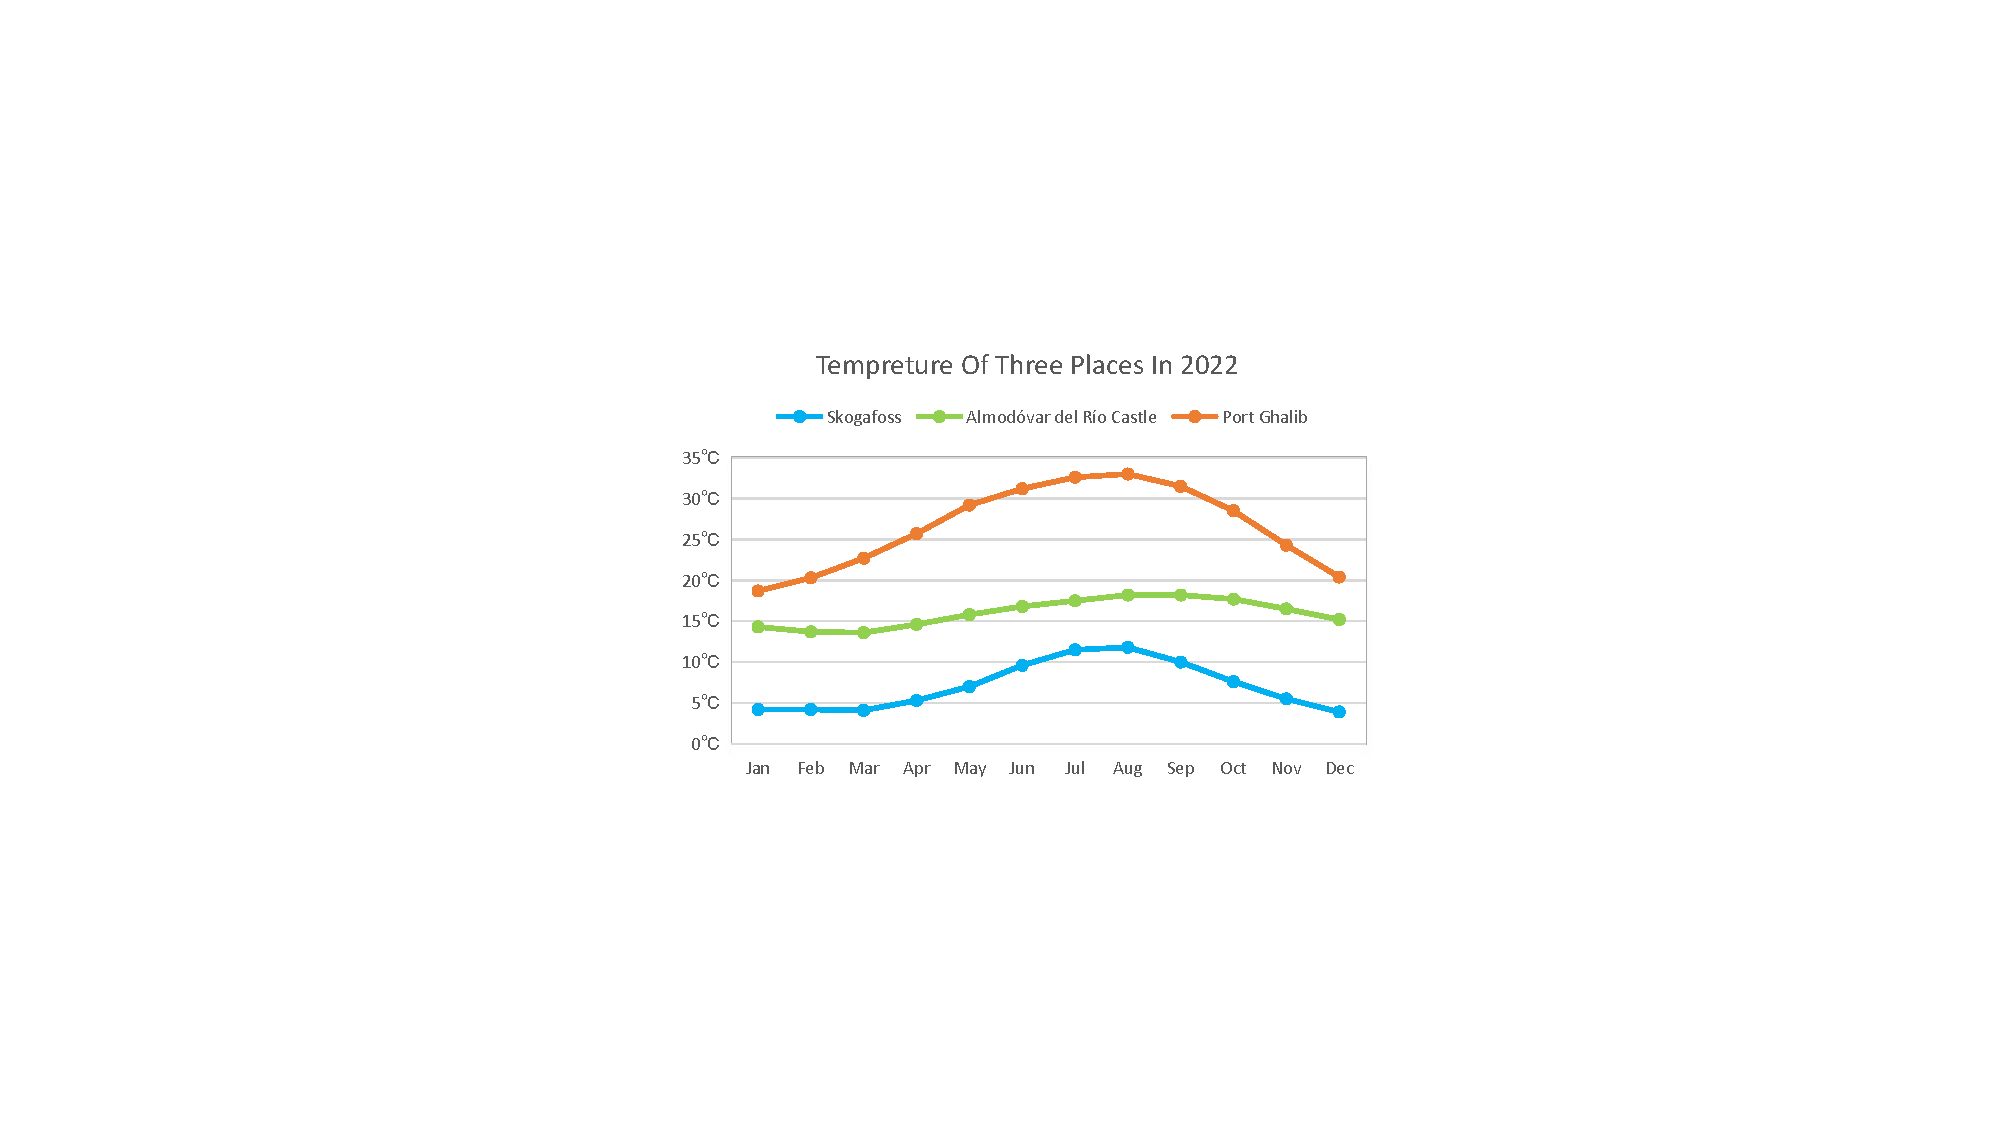
\includegraphics[width=1\textwidth]{tempreture.pdf}
		\caption{tempreture of pastureland}\label{fig:quanju}
	\end{minipage}
	\begin{minipage}[t]{0.3\textwidth}
		\centering
		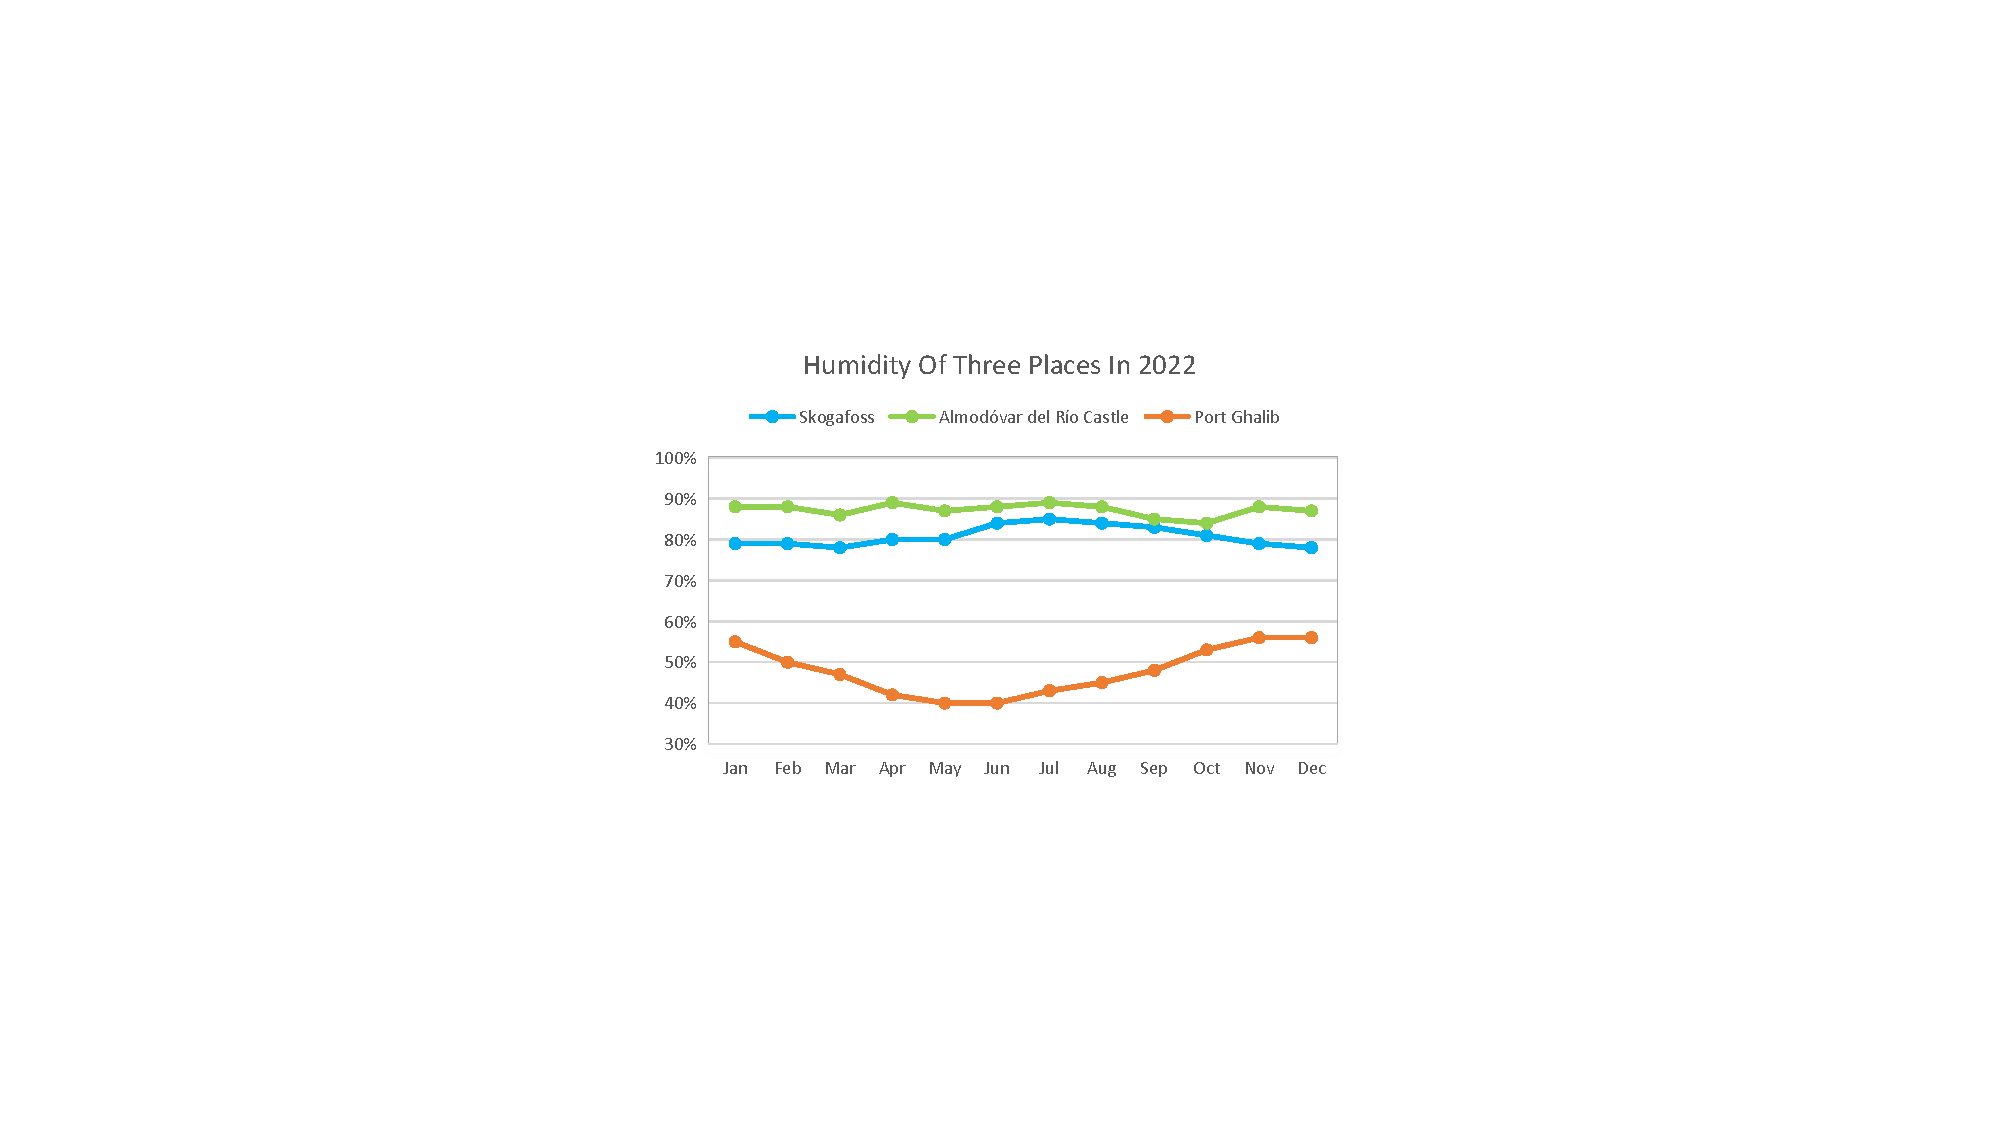
\includegraphics[width=0.98\textwidth]{humidity.pdf}
		\caption{humidity of pastureland}\label{fig:jubu}
	\end{minipage}
 	\begin{minipage}[t]{0.3\textwidth}
		\centering
		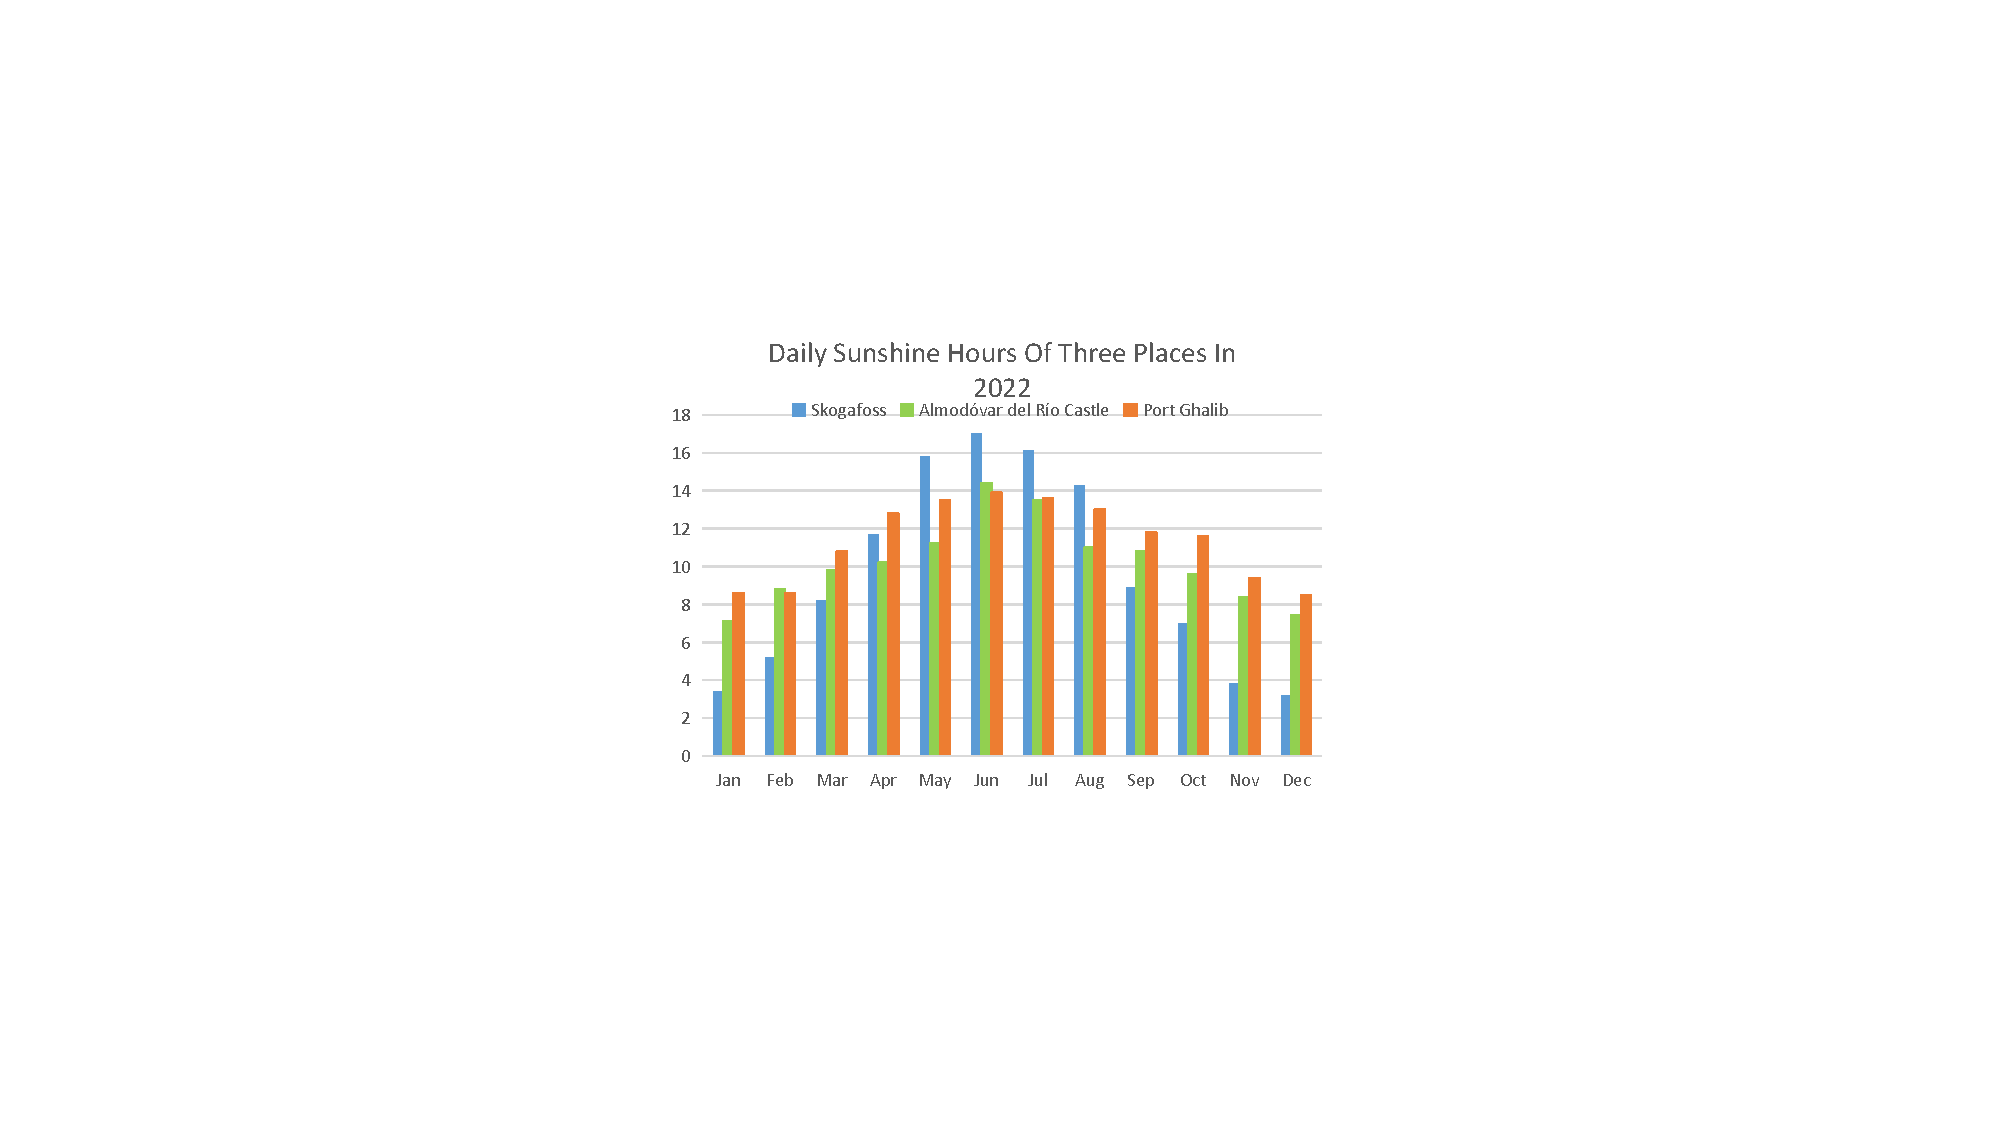
\includegraphics[width=0.98\textwidth]{sunlight.pdf}
		\caption{sunlight of pastureland}\label{fig:jubu}
	\end{minipage}
\end{figure}

Given the limited flying distance of the dragon, we chose three representative pastures within the limited range of longitude. The breeders can domesticate the dragons in one of the three pastures according to their needs. All pastures are capable of raising sheep on a large scale.


The temperature and light in the three pastures showed seasonal variation and reached the maximum in summer. As far as humidity indicators are concerned, the tropical Port Ghalib has the lowest humidity in summer, while the other two ranches maintain an equilibrium of humidity throughout the year (80-90\%). According to \eqref{eq:eq20}, we modified the growth coefficient of herbage, the feeding coefficient of dragon and the maximum saturated yield of sheep and grass in the pasture-sheep model,as shown in the following table:

\begin{table}[!htbp]
	\caption{Model parameter setting}
    \label{tab:table_two}
    \centering
	\begin{tabular}{ccccc}
\toprule
Pasture	&$r_1$&$N_1$&$N_2$&$m$	\\
		\midrule[0.75pt]
  	Port Ghalib & 0.58 & 58&10&0.02\\
 	Skogafoss & 0.68 & 68&20&0.005\\
 	Castle & 1 & 100&40&0.01\\
		\bottomrule[1.5pt]
	\end{tabular}
\end{table}


We averaged the temperature, humidity and light data to get the characteristic growth rates of different temperature zones. It can be clearly seen from the results that, from the aspect of forage yield, the humid temperate zone is greater than the arid zone than the cold zone, and the sheep yield is the same. This means that if you need the same number of sheep, you need more pasture area in dry and cold areas. In the case of domesticated dragons, however, a much smaller heat supply is needed in cold regions. But this is not conducive to the rapid growth of the dragon. In the tropics, dragons need more heat to maintain their resting metabolic rate, so they grow faster, but they need more energy. In the temperate zone, where the heat needs of dragons are moderate, local sheep production is the highest, and thus the most suitable for domesticating dragons.
 \newpage
\vspace{-0.3cm}
\begin{figure}[htbp]
	\centering
	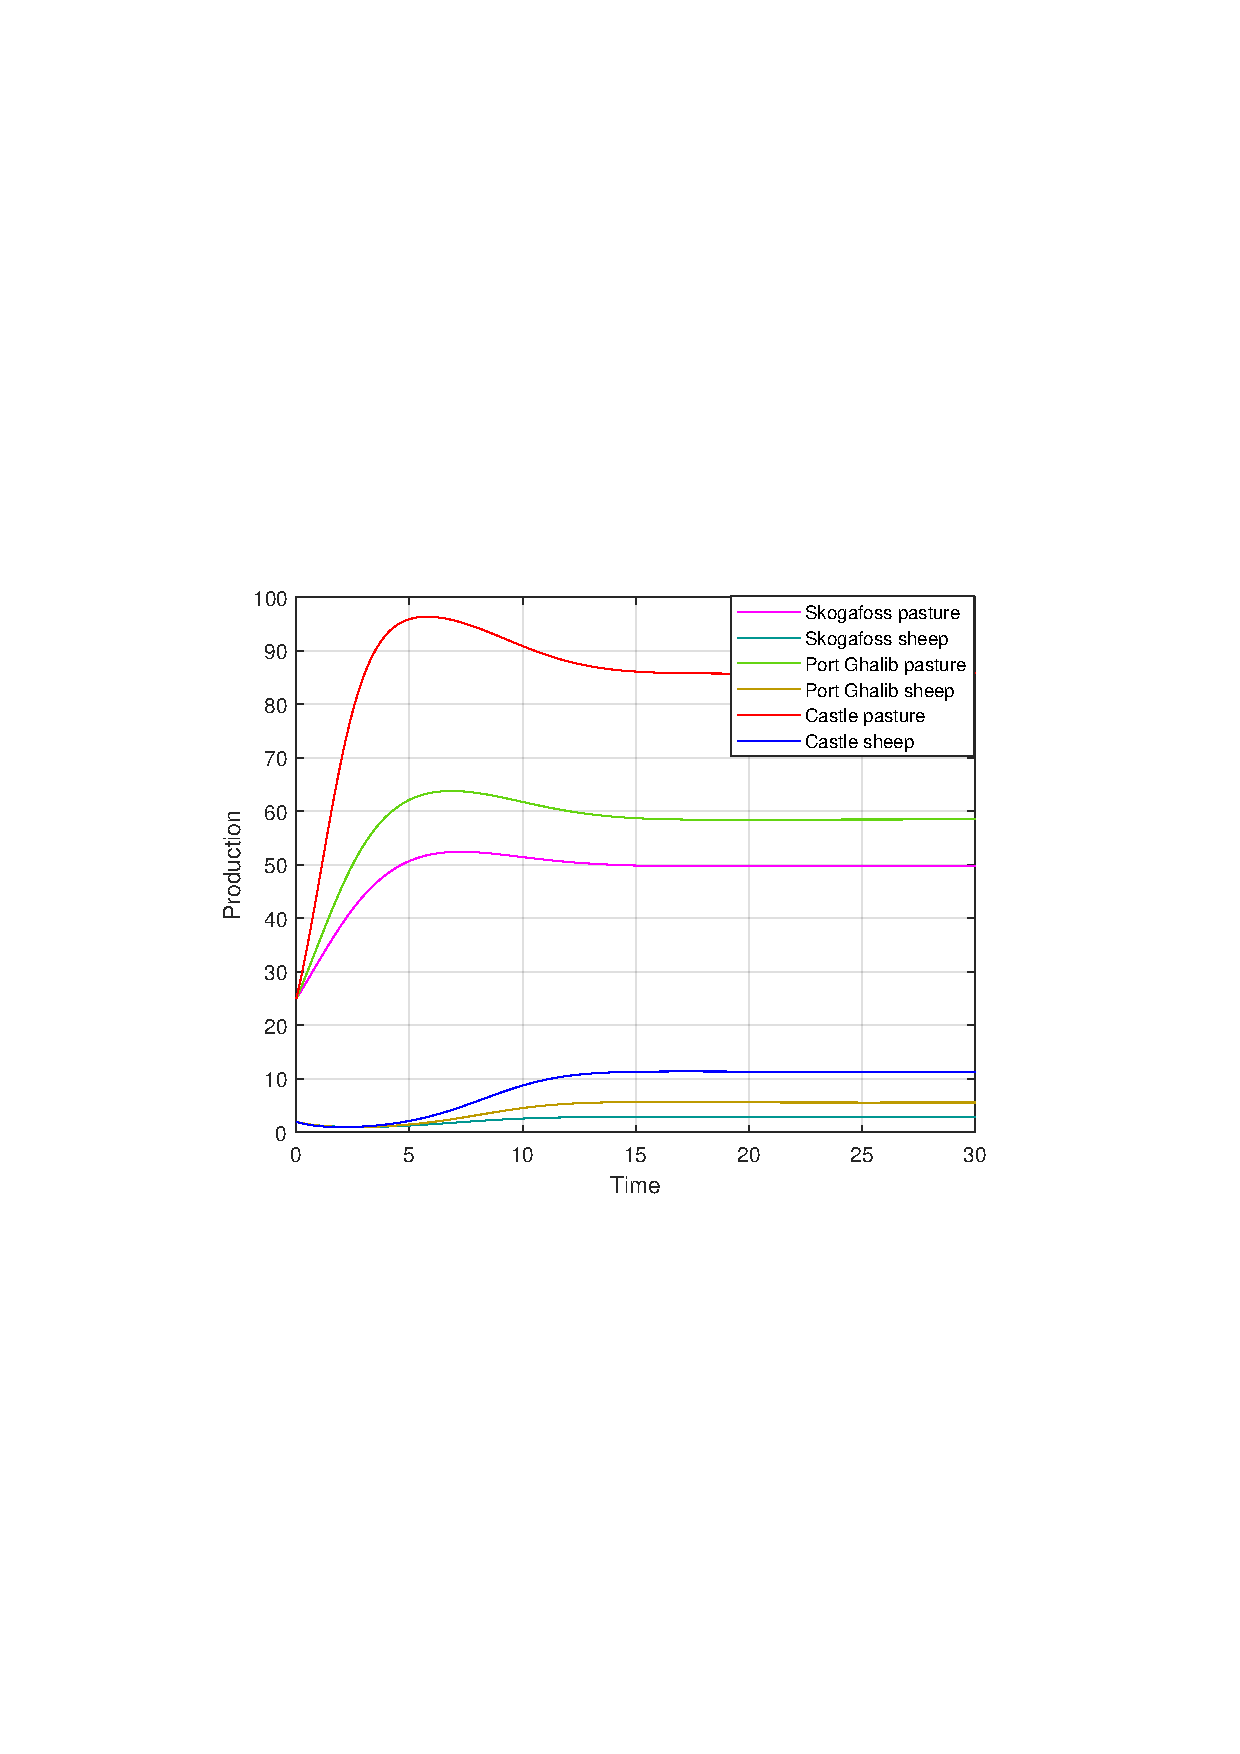
\includegraphics[width=0.45\textwidth]{3areasplot.pdf}
	\caption{Simulation results of three pastures}\label{fig:work1}
\end{figure}
\vspace{0.3cm}
 According to the different average temperatures in the three regions, the resting metabolic rate of the dragon will also change.Thus, in high temperature areas, dragons consume more energy and eat more sheep, that is, they need more grassland to provide services.It's shown in the figure below:

\vspace{-0.3cm}
\begin{figure}[h]
	\centering
	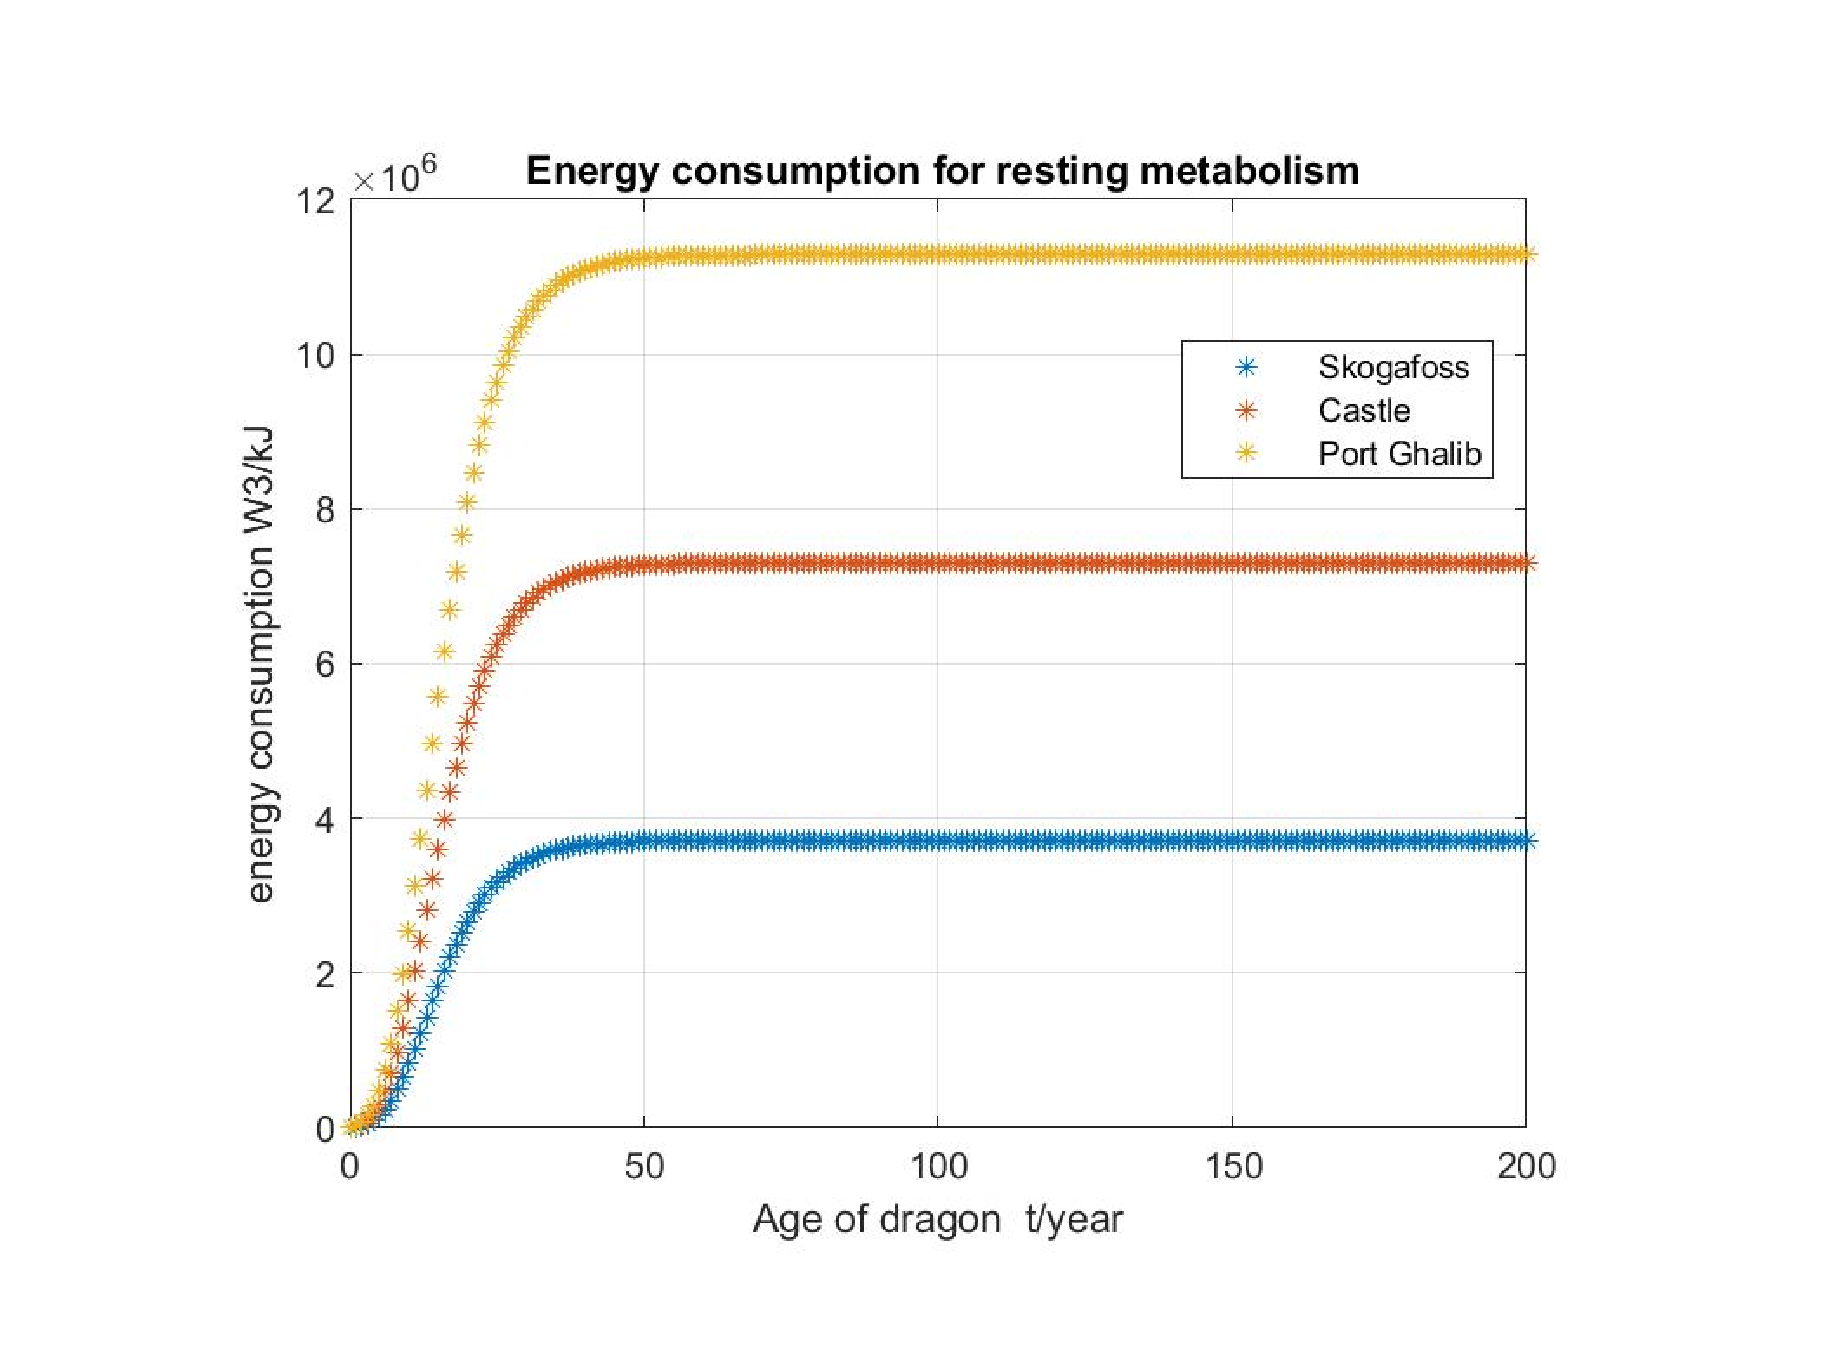
\includegraphics[width=0.6\textwidth]{easymcm/img/abcd.pdf}
	\caption{Energy consumption for resting metabolism}
\end{figure}
\vspace{-0.3cm}

\subsection{Dragon's service model}

In this section, we focus on the different ways dragons are used and the corresponding ways of serving them. Services include the area needed to domesticate the dragon, the preservation of the dragon's living space and the improvement of the dragon's habits.

First of all, an adult dragon weighs about 75$t$, roughly 468 times that of an adult Siberian tiger. We estimate the territory of adult dragons based on the territorial behavior of the Amur tiger, a solitary carnivore. It's roughly 14,000 $km^{2}$. We expand it slightly to a circle with a radius of 70$km$. All airspace in this circle is owned by the dragon.

Secondly, in order to ensure the safety of the Dragon, especially the surrounding people, we have set up a wider military control area 100$km$ more outside the Dragon's territory. There are guarded walls and regular helicopter patrols. Such treatment is beneficial to the safety of people's lives and the privacy of the dragon. Better yet, the dragon can become familiar with the surrounding military environment and gradually improve its living habits. This will increase their stability on the battlefield.
\vspace{-0.3cm}
\begin{figure}[htbp]
	\centering
	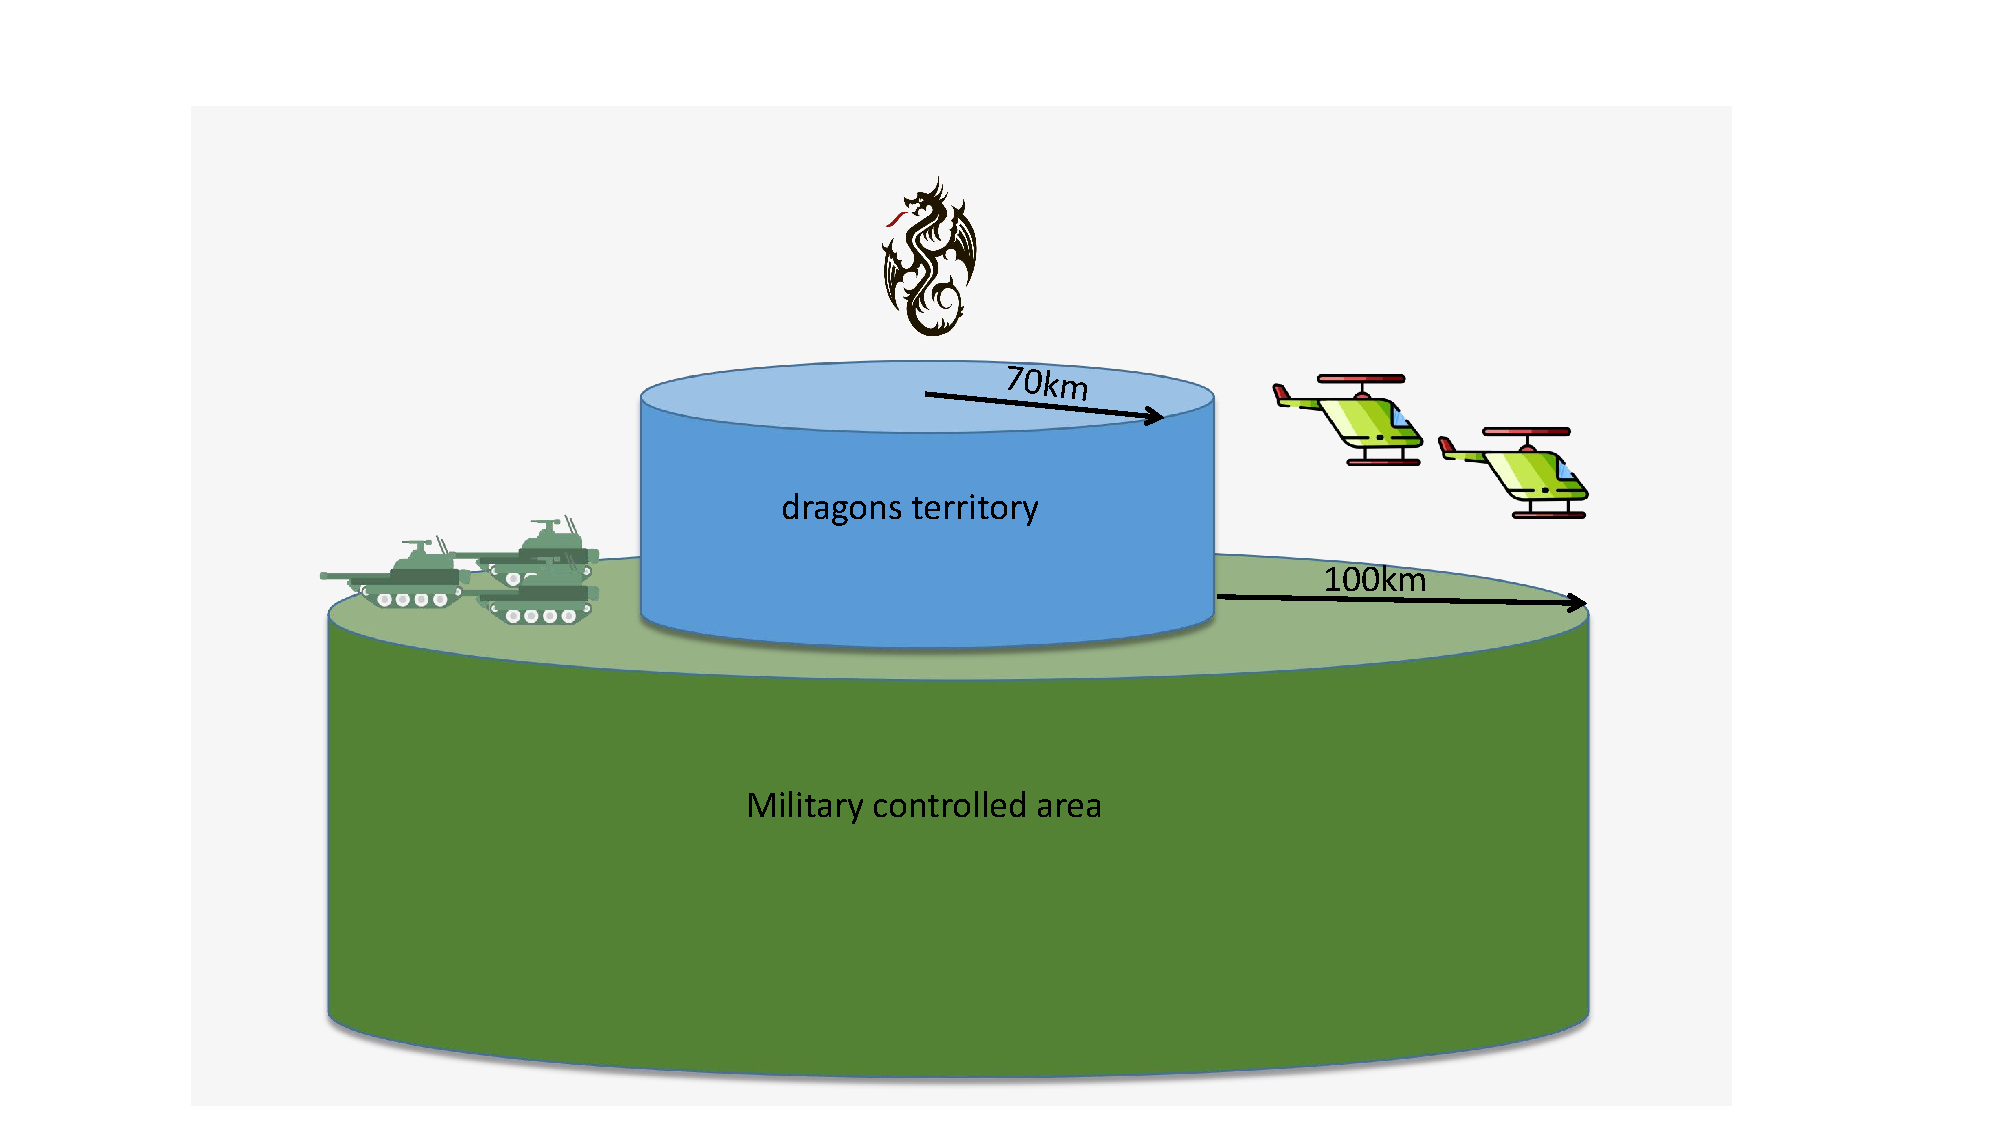
\includegraphics[width=0.7\textwidth]{easymcm/img/Domestication_area.pdf}
	\caption{Domestication area}\label{fig:work1}
\end{figure}

Next we discuss the two forms of dragon domestication, reproduction and warfare. For breeding dragons, we're set to fly for an hour a day, and fire breathing is only used for cooking lamb. In a war situation, we extend our flight time to 5-10 hours a day, spout fire, and have to recover from injuries. In this case, the dragon's consumption increases significantly, as shown in the chart below:

\begin{figure}[h]
	\centering
	\begin{minipage}[t]{0.45\textwidth}
		\centering
		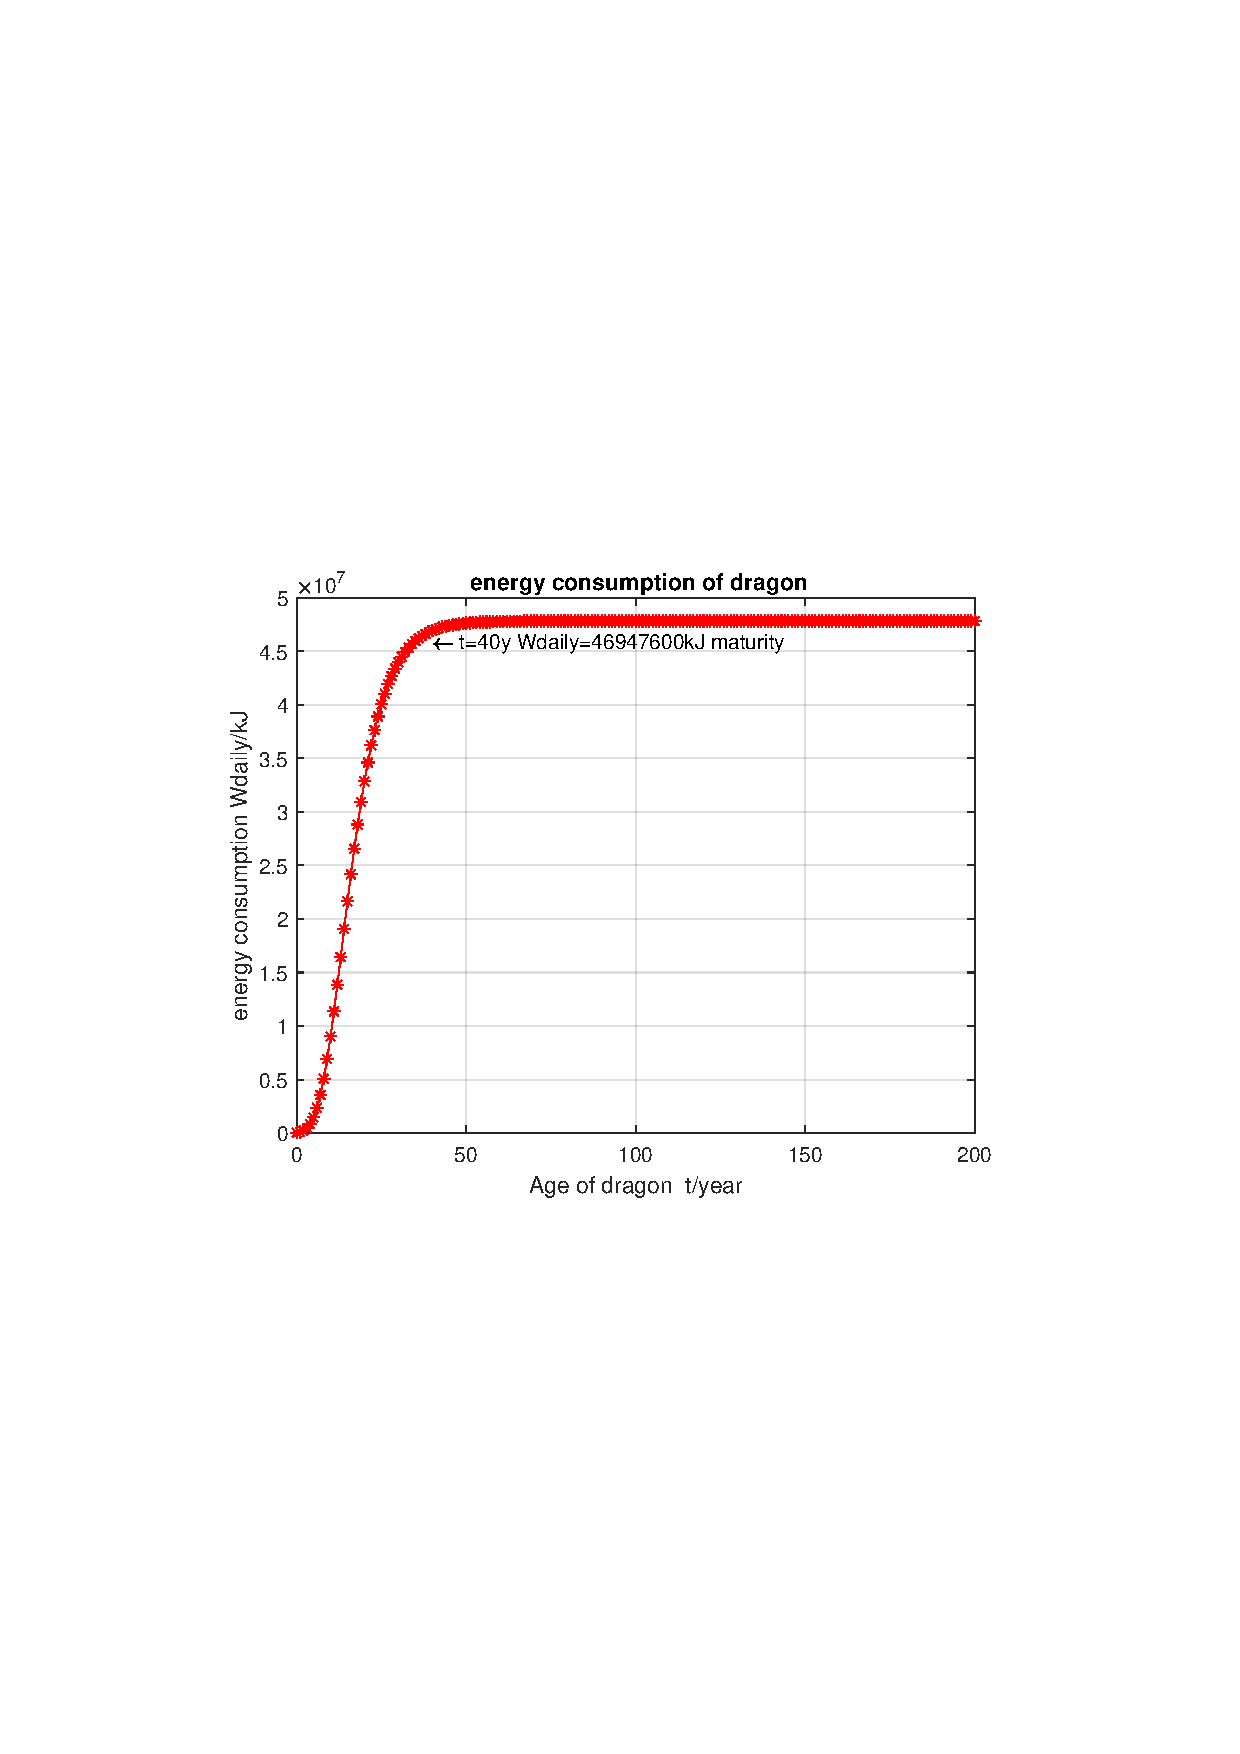
\includegraphics[width=1\textwidth]{energy consumption of dragon in war.pdf}
		\caption{energy consumption of dragon in war}\label{fig:quanju}
	\end{minipage}
	\begin{minipage}[t]{0.45\textwidth}
		\centering
		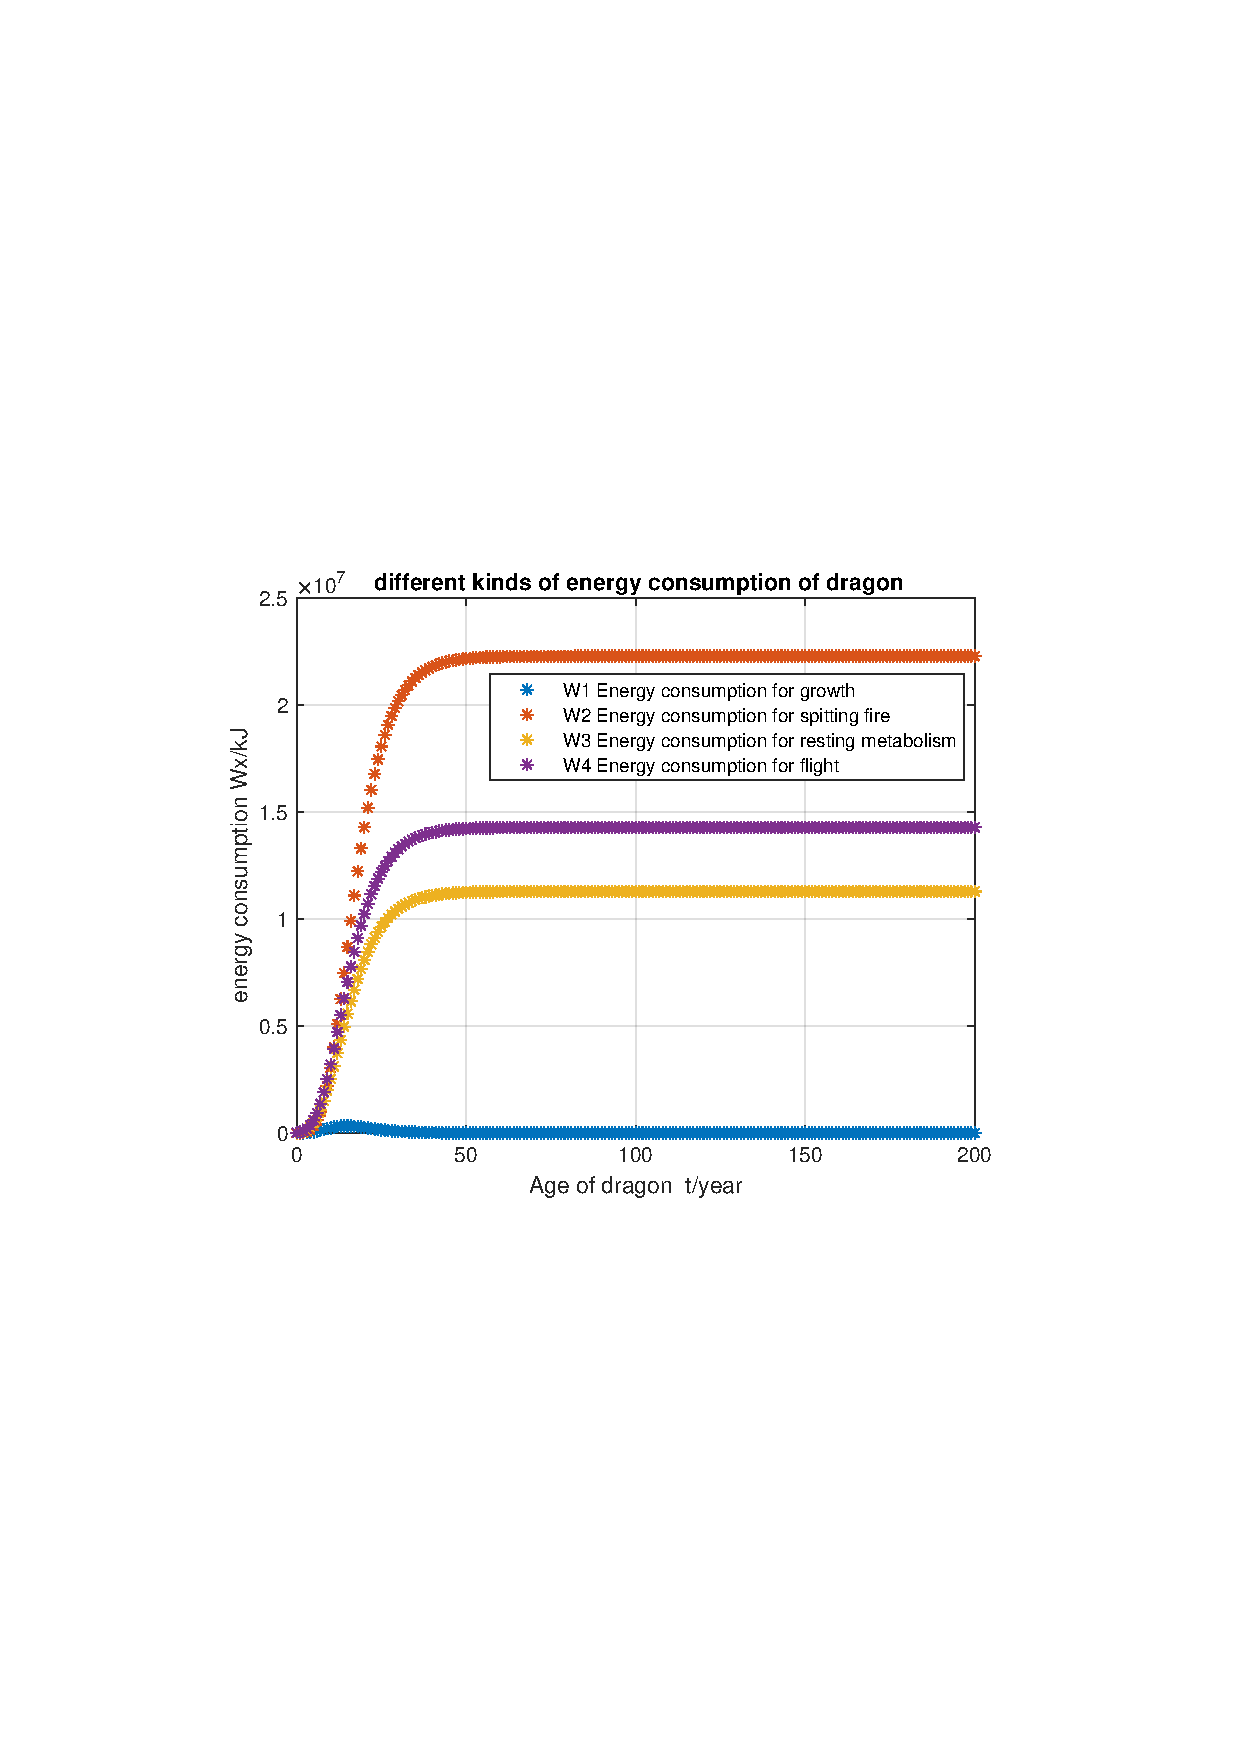
\includegraphics[width=0.98\textwidth]{different kinds of energy consumption of dragon in war.pdf}
		\caption{different kinds of energy consumption of dragon in war}\label{fig:jubu}
	\end{minipage}
\end{figure}

The two graphs above show the energy expenditure we obtained using model 1, and we can see that the energy expenditure reached $4.75\times10^7kJ$, which is about four times the original default survival state. The main expenditure of energy changes from resting metabolism to spitting fire. And the energy cost of flight is about four times that. So, in addition to the pasture that provides the sheep, we need to get other food as a new source of energy.

\section{Implementation}
\vspace{-0.3cm}



\subsection{Task 1\&2}
\vspace{-0.3cm}
Through literature research and watching videos of dragons on YouTube, we have determined that dragons possess the following characteristics: the ability to breathe fire with flames hot enough to melt iron thrones; a hard, scaly hide providing an extremely high level of protection; large size and weight, able to fly by flapping their wings to generate lift; a diet primarily composed of meat; constant growth throughout their lifetime; and a lifespan of up to 200 years.

Additionally, dragons are at the top of the food chain, and their role in the ecosystem is similar to that of tigers and leopards, mainly hunting herbivorous animals, thereby maintaining the balance of natural plants and grazing animals. The dragon's breath is mainly used to roast sheep, which may burn grasslands, but considering the relatively small area of impact, we believe that the dragon's active destruction of the environment can be ignored.

However, in the case of using dragons for warfare, their main impact would be the devastating destruction of enemy ecosystems. In this scenario, dragons would completely wipe out not just the herbivorous animals that they would normally prey on, but also the entire food chain from producers to consumers. Additionally, considering the extremely high temperatures of dragon fire, we believe that decomposers in the ecosystem would also be destroyed by the heat, leading to a very long time for the ecosystem to recover.

Due to the use of dragon flame and high intensity movement, the dragon's energy demands on our side will also increase significantly. If the area of our territory is not large enough, in other words, if it cannot provide enough energy, then it is very likely that we will consume the potential of the local ecosystem to meet temporary needs. This will also have a negative impact on the normal cycle of our ecosystem. But relatively speaking, this impact can be alleviated by expanding the area of our territory, and relatively speaking, our losses are always smaller than the enemy's ecosystem.
\subsection{Task 3}
\vspace{-0.3cm}
For the third question, what is the energy consumption of dragons,we considered the temperature, the amount of movement, the amount of fire and other factors. We have adopted Gompertz model for its weight accumulation, and obtained the energy needed for the daily growth of the dragon. We also assume that the fuel for the dragon fire is ethanol produced by the fermentation of the stomach, which obtains the energy required for the fire. After fitting and analyzing the static metabolic rate of lizards, we obtained the daily static metabolic rate of dragons. Through the force analysis of the dragon during flight, we get the expression of the daily flight energy consumption of the dragon. The sum of each item finally obtained the daily energy required by the dragon.

\subsection{Task 4\&5}
\vspace{-0.3cm}

Our answer to the question of how much area is needed to support three dragons is that each dragon needs a service area with a radius of 170km, of which the inner circle with a radius of 70km is the territory of the dragon, that is, the living area. The outer ring is the military control area, in which guard cards and troops should be set to ensure the privacy of the dragon and the life safety of the public. If each dragon can share territory, the service area can be further reduced.

In order to provide different levels of help to the dragon, our consideration is to divide the main state of the dragon into war and reproduction. Where the breeding state can be considered the default domestication scheme, we can use the design in the previous paragraph. In the state of war, in addition to letting the dragon learn modern military theory in peacetime, we also need to improve the dragon's energy supply and medical assistance. This requires the intervention of military academies and hospitals dedicated to dragons. Therefore, the cultivation of these two sectors is also within the scope of our plan.

\subsection{Task 6}
\vspace{-0.3cm}

As for the influence of climate conditions on our analysis, we have reached the conclusion in the previous article: in order to maximize national interests, dry and cold areas are not suitable for domesticating dragons, and warm and humid temperate or subtropical grasslands are the best choice. Unless for other reasons, dragons need to be familiar with dry or cold environments.



% \newpage
\section{Strengths and Weaknesses}
\vspace{-0.3cm}

\subsection{Strengths}
\vspace{-0.3cm}

\begin{itemize}

\item[$\bullet$] \textbf{Accurate Simulation }Our model, which employs the utilization of calories to quantify energy expenditure, effectively concretizes an otherwise abstract concept. Furthermore, in determining energy consumption through activities such as physical exertion and combustion, we employ scientifically rigorous modeling techniques to ensure the utmost precision in our calculations. Additionally, the weather data employed in our model was procured from official sources specific to the location in question, lending a robust practicality to our approach.

\item[$\bullet$] \textbf{Robust Model }As shown in our sensitivity analysis results, our model has strong robustness under both condition 1 and condition 2. Therefore, we believe that our model has good robustness.

\item[$\bullet$] \textbf{Strong Interpretability }In creating our model, we not only maintain a high level of respect and reference to the original works but also combine current world natural science laws to build the model, making the scenario of raising dragons as a magical animal as realistic as possible. For example, by comparing lizards with dragons, we analyze the thermoregulation characteristics of dragons and reference alcohol synthesis combustion to analyze the dragon's fire-breathing process. Through these means, we strive to give the scenario of raising dragons a more realistic sense and thus bring a highly interpretable model.

\item[$\bullet$] \textbf{Universality } Our model, which describes the interactions between dragon cultivation and the surrounding ecosystem, can not only provide insights into dragon-related scenarios, but also has practical applications in evaluating other segments of the ecosystem, such as sheep rearing. Furthermore, it serves as a valuable reference for the conservation of other apex predators of similar nature.

However, there are weaknesses in the proposed models:
\end{itemize}
\vspace{-1cm}
\subsection{Weaknesses}
\begin{itemize}

\item[$\bullet$] \textbf{Lack Of Real Data }The direct data we have on dragons primarily comes from television show stills and novel source material, however, obtaining data through this method is relatively limited. As a result, we have had to make a fair number of reasonable assumptions and inferences based on scientific facts. This also results in our model deviating from the dragons as imagined by the original authors.

\item[$\bullet$] \textbf{Limited Food Variety }Due to time constraints, we only kept beef and mutton in the dragon's diet, while according to the original work, dragons would also eat many other foods including fish. Therefore, if we consider seafood such as fish and shrimp, we will get different results under specific conditions. For example, in the Arctic, it may be possible to feed dragons by breeding krill, which is certain to make some difference to our current conclusions.


\end{itemize}

\\
\\
\\
\begin{thebibliography}{99}
	\vspace{-0.5cm}
	\bibitem{1} Hamilton, A. J., et al. (2015). "Here be dragons." Nature 520(7545): 42-43.
    \bibitem{2} Hogarth, P. J. (1976). "The ecology of dragons: a reply." Nature 264(5587): 607-607.
    \bibitem{3} L, R. (1901). "Dragons of the Air: an Account of Extinct Flying Reptiles." Nature 64(1670): 645-646.
    \bibitem{4} Scamander, N. Fantastic Beasts and Where to Find Them (Bloomsbury, 2001).
    \bibitem{5} Michel JB, Quantitative analysis of culture using millions of digitized books. Science. 2011 Jan 14;331(6014):176-82.
	\bibitem{6} Selden, D. (2010). Resurrecting the Red Dragon: A Case Study in Welsh Identity [Master's thesis, Ohio University]. 
    \bibitem{7} Wagner R. The ring of the Nibelung[M]. WW Norton \& Company, 1977.
    \bibitem{8} Williams M. King Arthur in history and legend[J]. Folklore, 1962, 73(2): 73-88.
    \bibitem{9} Gough J. Tolkien's Creation Myth in" The Silmarillion"--Northern or Not?[J]. Children's Literature in Education, 1999, 30(1): 1-8.
    \bibitem{10}\url{https://en.wikipedia.org/wiki/List_of_A_Song_of_Ice_and_Fire_characters}
    \bibitem{11}\url{https://en.wikipedia.org/wiki/A_Song_of_Ice_and_Fire}
    \bibitem{12}\url{https://faunalytics.org/global-animal-slaughter-statistics-charts-2022-update}
    \bibitem{13}J. Teleken, A. C. Galvão, W. S. Robazza
     Comparing non-linear mathematical models to describe growth of different animals
 . 7 February 2017. Animal Sciences
    \bibitem{14}Xu Yi.Effects of temperature on metabolic rate, heart rate and respiratory rate of adult desert lizard influence .2014.12. Journal of Lanzhou University (Natural Sciences)
    \bibitem{15}Estimating power curves OF flying vertebrates. Jeremy M. V. Rayner. 21 September. WWW 16 November 1999
\bibitem{16} Chen X, Zhang H, Yao X, et al. Latitudinal and depth patterns of soil microbial biomass carbon, nitrogen, and phosphorus in grasslands of an agro‐pastoral ecotone[J]. Land Degradation \& Development, 2021, 32(14): 3833-3846.
    \bibitem{17} Jiao C, Yu G, He N, et al. Spatial pattern of grassland aboveground biomass and its environmental controls in the Eurasian steppe[J]. Journal of Geographical Sciences, 2017, 27: 3-22.
    \bibitem{18} Chen L, Li H E, Zhang P, et al. Climate and native grassland vegetation as drivers of the community structures of shrub-encroached grasslands in Inner Mongolia, China[J]. Landscape Ecology, 2015, 30: 1627-1641.
    \bibitem{19} Yao Z, Xin Y, Yang L, et al. Precipitation and temperature regulate species diversity, plant coverage and aboveground biomass through opposing mechanisms in large-scale grasslands[J]. Frontiers in Plant Science, 2022, 13.

    \bibitem{20} Zeng Yajie, Xu Jiliang, Li Yanchun,et al. Research progress of nature reserve area and wildlife space requirements [J]. World Forestry Research, 2010 (4): 46-50. 

    \bibitem{21} Zhang Meiling, Chen Quan-gong, JIANG Wen-lan,et al. Simulation and sensitivity analysis of net Primary productivity (NPP) of different grassland types [J]. Arid Land Geography, 2021, 44(2): 369-378.

    
\end{thebibliography}



% 以下为信件/备忘录部分,不需要可自行去掉
% 如有需要可将整个 letter 环境移动到文章开头或中间
% 请在后一个花括号内填写信件(Letter)或备忘录(Memorandum)标题
\begin{letter}{Letter\centering}
	\begin{flushleft}  % 左对齐环境,无首行缩进
		\textbf{To:} \textbf{George R.R. Martin}\\
		\textbf{From:} \textbf{Team 2308932}\\
		\textbf{Date:} \textbf{February 19th, 2023}\\
		\textbf{Subject:} \textbf{Game of Ecology}
	\end{flushleft}

\noindent Dear Mr.Martin:

 We are big fans of your book \textit{A Song of Ice and Firez} and the legends in your story fascinate us deeply. o, it is a great honor for us to write to you about our scheme concerning bringing Khaleesi's three dragons into our world. This is an exciting adventure, and we welcome you to look through our exploration of a such challenging task. We believe our efforts can assist you to get a deeper insight into how to maintain the realistic ecological underpinning of the story.

 Our primary focus is on understanding how to measure the characteristics, behaviors, habits, diet, and interactions of dragons with the environment. To address this, we have established a model for the energy metabolism of dragons. This model primarily takes into account the innate characteristics of the dragon such as age, volume, and its behavior needs such as flying and breathing fire, as well as the impact of external factors such as temperature. Based on this, we have developed a formula that can measure the energy needed by a dragon in a day. This result will serve as the foundation for our further exploration.

 
 we focus on the different ways dragons are used and the corresponding ways of serving them. Services include the area needed to domesticate the dragon, the preservation of the dragon's living space and the improvement of the dragon's habits.

 First of all, an adult dragon weighs about 75$t$, roughly 468 times that of an adult Siberian tiger. We estimate the territory of adult dragons based on the territorial behavior of the Amur tiger, a solitary carnivore. It's roughly 14,000 $km^{2}$. We expand it slightly to a circle with a radius of 70$km$. All airspace in this circle is owned by the dragon.

Secondly, in order to ensure the safety of the Dragon, especially the surrounding people, we have set up a wider military control area 100$km$ more outside the Dragon's territory. There are guarded walls and regular helicopter patrols. Such treatment is beneficial to the safety of people's lives and the privacy of the dragon. Better yet, the dragon can become familiar with the surrounding military environment and gradually improve its living habits. This will increase their stability on the battlefield.

Well, to tell the truth, we encountered such a problem when we tried to analyze how to evaluate how much resource and space is enough to feed the three brothers, as there is no direct data that can tell us their diet or living habits. So we come up with an idea: We decided to do subtraction. To be exact, we followed Khaleesi's decision in your story and served the dragons only with sheep in our modules. The advantage of this measure locates at the focus is shifted from how to make direct connection between the dragon and space calculation to the consideration of the balance between large numbers of sheep and the environment.
Under this theory guide, we established our second module: pasture growth model. This module mainly concerns factors
 like sunlight, temperature, and humidity that affect the growth of grass. What's more, we bride the dragons' energy metabolism with this module, which makes it possible for us to give a precise result about how to raise the three dragons in our real world from not only the aspects of objective factors like climate, but subjective choices like launching a war.
\begin{flushright}
\textit{Growing Strong}

 Your Faithful Readers
\end{flushright}

\end{document}  % 结束